%FOR PDFLATEX USE ONLY
\documentclass[a4paper,14pt]{article}

\usepackage{amssymb,amsmath} %math symbols

\usepackage[margin=2cm, bottom=2cm]{geometry} %paper geometry

\usepackage[utf8]{inputenc} %allows unicode (including russian) source file
\usepackage[russian]{babel} %docment in russian-style
\usepackage[utf8]{inputenc}
\usepackage[unicode]{hyperref} %links inside of the text
\usepackage[pdftex]{graphicx} %includegraphics pictures
\usepackage{cmlgc} %bold text

\usepackage{array} %arrays

\usepackage{cancel}
\usepackage{wrapfig}
\usepackage{array}
\usepackage{lipsum}
\usepackage{esvect}
\usepackage{longtable}
\usepackage{verbatim} 
\usepackage{multirow}
\usepackage{hyperref}
\usepackage{mathtools}
\usepackage{subfig}
\usepackage{calc}
\usepackage{pgfplots,tikz,circuitikz}
\usepackage{tkz-euclide}
\usepackage{gensymb}
\usepackage{bm}

\newenvironment{changemargin}[2]{%
\begin{list}{}{%
\setlength{\topsep}{0pt}%
\setlength{\leftmargin}{#1}%
\setlength{\rightmargin}{#2}%
\setlength{\listparindent}{\parindent}%
\setlength{\itemindent}{\parindent}%
\setlength{\parsep}{\parskip}%
}%
\item[]}{\end{list}}

\newcommand{\specialcell}[2][c]{%
  \begin{tabular}[#1]{@{}c@{}}#2\end{tabular}}
%\newenvironment{comment}{}{}

\begin{document}

\begin{center}
	\LARGE{\textbf{Кооперативная работа по практике научных семинаров.}}
\end{center}

\begin{center}
	\normalsize{Архипов Павел Александрович, Балакшин Артур Вячеславович, Бойцов Евгений Георгиевич, Варламов Антоний Михайлович, Ведерников Роман Алексеевич, Гаврилов Дмитрий Сергеевич, Гладышева Анна Антоновна, Денисов Яков Русланович, Князев Фёдор Алексеевич, Коковин Артём Дмитриевич, Кулешов Станислав Эдуардович, Лёвин Андрей Валерьевич, Малиновский Владимир Валерьевич, Натаров Илья Игоревич, Павлов Михаил Михайлович, Панферов Андрей Денисович, Полянский Артём Максимович, Рева Максим Андреевич, Сафонова Елизавета Александровна, Сыроваткин Степан Михайлович, Царёв Дмитрий Вячеславович, Яушев Михаил Олегович}
\end{center}

\section*{1.3}
\begin{center}
	\LARGE{\textbf{Список элементарных частиц.}}
\end{center}


В этом пункте мы рассмотрим элементарные частицы стандартной модели обнаруженные и предсказаные.

Их можно условно разделить на три класса:

\subsection*{Вещество}

\subsubsection*{Кварки}

Кварки участвуют в сильных, слабых, электромагнитных и гравитационных взаимодействиях. Сильные взаимодействия (обмен глюоном) могут изменять цвет кварка, но не меняют его аромат. Слабые взаимодействия, наоборот, не меняют цвет, но могут менять аромат. Кварки имеют античастицы, обладающие такой же массой и обратным зарядом. Все кварки обладают спином $1/2$.Необычные свойства сильного взаимодействия приводят к тому, что одиночный кварк не может удалиться на какое-либо существенное расстояние от других кварков, а значит, кварки не могут наблюдаться в свободном виде. Математический аппарат теории кварков основан на экспериментально подтверждённом предположении, что взаимодействия кварков инвариантны относительно группы изоспиновых преобразований $SU(3)$.

\begin{center}
\begin{tabular}{|c|c|c|}
\hline
Символ кварка/антикварка (аромат)&Масса&заряд\\
\hline
$u/\overline{u}$&$1.5 \tilde 3$&+2/3\\
\hline
$d/\overline{d}$&$4.79 \pm 0.07$&-1/3\\
\hline
$c/\overline{c}$&$1250 \pm 90$&+2/3\\
\hline
$s/\overline{s}$&$95 \pm 25$&-1/3\\
\hline
$t/\overline{t}$&$174340 \pm 790$&+2/3\\
\hline
$b/\overline{b}$&$4200 \pm 70$&-1/3\\
\hline
\end{tabular}
\end{center}

\subsubsection*{Лептоны}

Лептоны не участвуют в сильном взаимодействии. Они также обладают античастицами с противоположным зарядом и такой же массой. Все лептоны обладают спином $1/2$. Каждому заряженному лептону соответствует лёгкий нейтральный лептон — нейтрино. Ранее считалось, что каждое поколение лептонов обладает своим флейворным лептонным зарядом, — иными словами, лептон может возникнуть только вместе с антилептоном из своего поколения, так, чтобы разность количества лептонов и антилептонов каждого поколения в замкнутой системе была постоянной. Эта разность называется электронным, мюонным или тау-лептонным числом, в зависимости от рассматриваемого поколения. Лептонное число лептона равно $+1$, антилептона — $-1$. С открытием осцилляций нейтрино обнаружено, что это правило нарушается: электронное нейтрино может превратиться в мюонное или тау-нейтрино и т. д. Таким образом, флейворное лептонное число не сохраняется.

\begin{center}
\begin{tabular}{|c|c|c|}
\hline
Название&Заряд&Масса (МэВ)\\
\hline
Электрон&-1&0.511\\
\hline
Мюон&-1&105.66\\
\hline
Тау-лептон&-1&1776.99\\
\hline
Электронное нейтрино&0&$<2.2 \cdot 10^{-6}$\\
\hline
Мюонное нейтрино&0&<0.17\\
\hline
Тау-нейтрино&0&<15.5\\
\hline
\end{tabular}
\end{center}

\subsection*{Переносчики взаимодействия}

Частицы переносчики четырех фунламентальных взаимодействий. 
\begin{center}
\begin{tabular}{|c|c|c|c|c|}
\hline
Название&Заряд (е)&Спин&Масса (ГэВ)&Переносимое взаимодействие\\
\hline
Фотон&0&1&0&Электромагнитное\\
\hline
$W^{\pm}$&$\pm 1$&1&80.4&Слабое взаимодействие\\
\hline
$Z^0$&0&1&91.2&Слабое взаимодействие\\
\hline
Глюон&0&1&0&Сильное взаимодействие\\
\hline
Бозон Хиггса&0&0&$\approx 125.09 \pm 0.24$&Инертная масса\\
\hline
Гравитон?&0&2&0&Гравитация\\
\hline
\end{tabular}
\end{center}

Гравитон является гипотетической частицей. Попытки расширить Стандартную модель гравитонами сталкиваются с серьёзными теоретическими сложностями в области высоких энергий (равных или превышающих планковскую энергию) из-за расходимостей квантовых эффектов. Решение этих вопросов было мотивом построения нескольких предложенных теорий квантовой гравитаци.

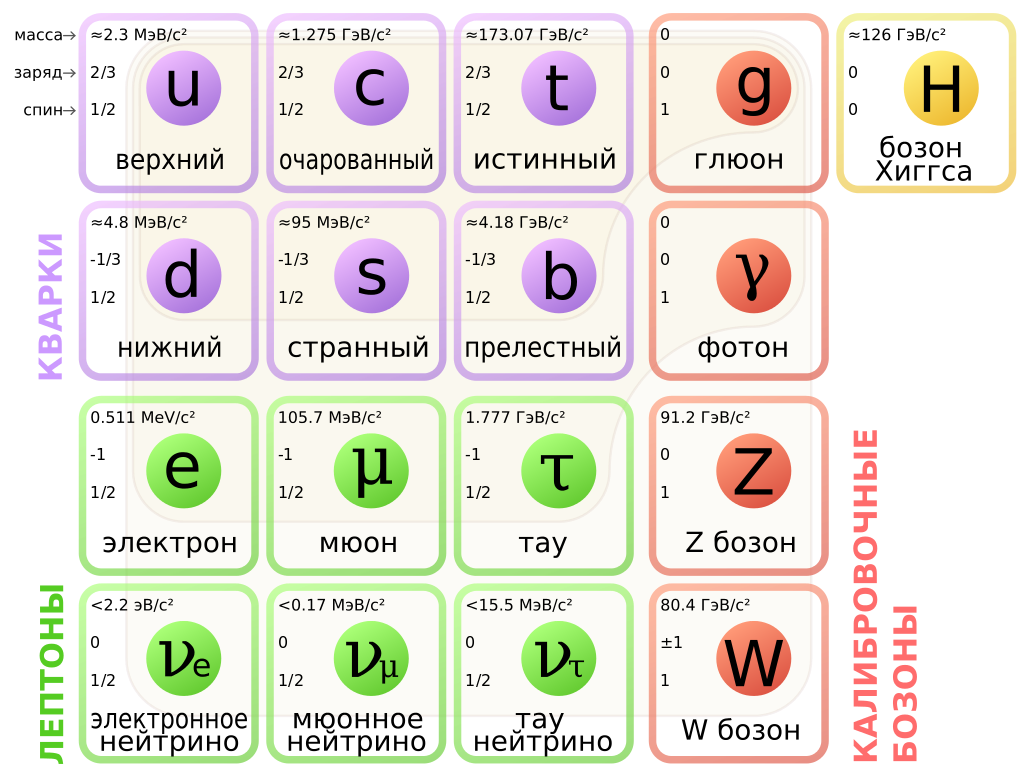
\includegraphics[width=1\textwidth]{basic_particles.png}


\section*{1.4}
\begin{center}
	\LARGE{\textbf{Последовательность событий в космологии.}}
\end{center}
\begin{center}
	Возраст вселенной по разным данным $13.75 \pm 0.13$ (WMAP) или $13.81 \pm 0.06$ (Planck) гигалет.
\end{center}
\begin{center}
\begin{longtable}{|c|c|c|}
\hline
 Время& Эпоха& События\\
\hline
 0& Сингулярность& Большой взрыв\\
\hline
 0 — $10^{-43}$ с& Планковская эпоха& Рождение частиц\\
\hline
 $10^{-43}$ — $10^{-35}$ с & \specialcell{Эпоха Великого\\объединения}& \specialcell{Отделение гравитации от\\ объединённого электрослабого\\ и сильного взаимодействия.\\ Возможное рождение\\ монополей. Разрушение\\ Великого объединения.} \\
\hline
 $10^{-35}$ — $10^{-32}$ с& Инфляционная эпоха& \specialcell{Вселенная экспоненциально\\ увеличивает свой радиус на\\ много порядков. Структура\\ первичной квантовой\\ флуктуации, раздуваясь, даёт\\ начало крупномасштабной\\ структуре Вселенной.\\ Вторичный нагрев.} \\
\hline
 $10^{-32}$ — $10^{-12}$ с& Электрослабая эпоха& \specialcell{Вселенная заполнена кварк-\\глюонной плазмой, лептонами,\\ фотонами, W- и Z-бозонами,\\ бозонами Хиггса. Нарушение\\ суперсимметрии.} \\
\hline
 $10^{-12}$ — $10^{-6}$ с& Кварковая эпоха& \specialcell{Электрослабая симметрия\\ нарушена, все четыре\\ фундаментальных\\ взаимодействия существуют\\ раздельно. Кварки ещё не\\ объединены в адроны.\\ Вселенная заполнена кварк-\\глюонной плазмой, лептонами и\\ фотонами.} \\
\hline
 $10^{-6}$ — 100 с& Адронная эпоха& \specialcell{Адронизация. Аннигиляция\\ барион-антибарионных пар.\\ Благодаря CP-нарушению\\ остаётся малый избыток\\ барионов над антибарионами\\ (около 1:$10^9$).} \\
\hline
 100 секунд — 3 минуты& Лептонная эпоха& \specialcell{Аннигиляция лептон-\\антилептонных пар. Распад\\ части нейтронов. Вещество\\ становится прозрачным для\\ нейтрино.} \\
\hline
 3 минуты — 380 000 лет& Протонная эпоха& \specialcell{Нуклеосинтез гелия, дейтерия,\\ следов лития-7 (20 минут).\\ Вещество начинает\\ доминировать над излучением\\ (70 000 лет), что приводит к\\ изменению режима расширения\\ Вселенной. В конце эпохи (380\\ 000 лет) происходит\\рекомбинация водорода и\\ Вселенная становится\\ прозрачной для фотонов\\ теплового излучения.} \\
\hline
 380 000 — 550 млн лет& Тёмные века& \specialcell{Вселенная заполнена\\ водородом и гелием,\\ реликтовым излучением,\\ излучением атомарного\\ водорода на волне 21 см.\\ Звёзды, квазары и другие яркие \\источники отсутствуют.} \\
\hline
 (550 — 800) млн лет& Реионизация& \specialcell{Образуются первые звёзды\\ (звёзды популяции III), квазары,\\ галактики, скопления и\\ сверхскопления галактик.\\ Реионизация водорода светом\\ звёзд и квазаров.} \\
\hline
 (0.8 — 8.9) млрд лет& Эра вещества& \specialcell{Образование межзвёздного\\ облака, давшего начало\\ Солнечной системе.} \\
\hline
 (8.9 — 9.1) млрд лет& Эра вещества& \specialcell{Образование Земли и других\\ планет нашей Солнечной\\ системы, затвердевание пород.} \\
\hline
\end{longtable}
\end{center}

\section*{1.5}
\begin{center}
	\LARGE{\textbf{Почему орбиты планет замкнуты?}}\\
\end{center}

Нахождение орбиты планеты - это задача о движении тела "вокруг" другого, более массивного неподвижного тела, иначе говоря, частицы во внешнем поле, потенциал которой зависит только от расстояния $r$ до определенной неподвижной точки, координаты которой задаются положением массивного тела в простарстве, такое поле называется \textit{центральным}. Сила
\begin{equation}\label{eq1}
\textbf{F} = -\frac{\partial U(r)}{\partial\textbf{r}} = \frac{dU}{dr} \frac{\textbf{r}}{r}
\end{equation}  
Момент ипульса в такой системе сохраняется, т.е. является интегралом движения:
\begin{equation}\label{eq2}
\textbf{M} = [\textbf{rp}]
\end{equation}
Векторы \textbf{M} и \textbf{r} взаимно перпендикулярны, то \textbf{r} всегда лежит в одной и той же плоскости, то есть траектория движения частицы в центральном поле лежит в одной плоскости.
Введя полярные координаты r и $\phi$, запишем функцию Лагранжа:
\begin{equation}\label{eq3}
L = \frac{m}{2}\left(\dot{r}^2 + r^2 \dot{\varphi}^2\right) - U(r)
\end{equation}
Заметим, что $\varphi$ не входит в явном виде в лагранжеву функцию, поэтому такая обобщенная координата является \textit{циклической} и, в силу уравнения Лагранжа:
\begin{equation}\label{eq4}
\frac{d}{dt} \frac{\partial L}{\partial \dot{\varphi}} = \frac{\partial L}{\partial \varphi} = 0
\end{equation} 
 соответсвующий $p_\varphi = \frac{\partial L}{\partial \dot{\varphi}}= mr^2\dot{\varphi}$ является интегралом движения. Опуская дальнейшие преобразования, мы можем получить зависимость $\varphi(\textbf{r})$:
\begin{equation}\label{eq5}
\varphi = \int \frac{(M/r^2)dr}{\sqrt{2m[E-U(r)] - (M^2/r^2)}} + const,
\end{equation}
где $M = mr^2\dot{\varphi}$ - момент импульса, $E = \frac{m\dot{r}^2}{2} + \frac{M^2}{2mr^2} + U(r)$ - энергия системы.
Стоит заметить, что движение ограничено значениями $r$, при которых $\dot{r} = 0$ (переход от уменьшения к увеличению радиус-вектора и наоборот). Если траектория ограничена $r_\text{min} \leq r$, то она \textit{инфинитна}, если же $r_\text{min} \leq r \leq r_\text{max}$ - она \textit{финитна}. Однако, финитность траектории совсем не означает ее замкнутость. За время, пока радиус-вектор изменяется от $r_\text{min}$ к $r_\text{max}$ и наоборот, $\textbf{r}$ повернется на:
\begin{equation}\label{eq6}
\Delta \varphi = 2 \int_{r_{min}}^{r_{max}} \frac{(M/r^2)dr}{\sqrt{2m[E-U(r)] - (M^2/r^2)}}  
\end{equation}


\begin{center}
        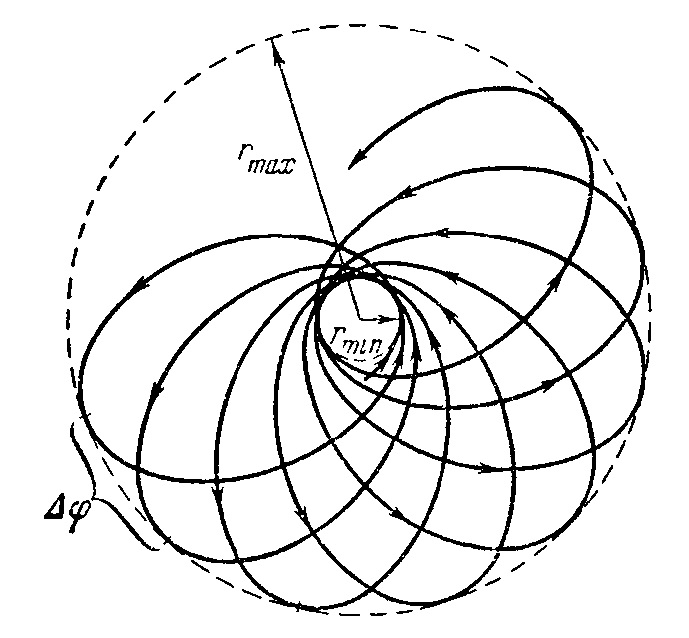
\includegraphics[width=0.5\textwidth]{1.jpg}
\end{center}
Чтобы орбита замыкалась, $\Delta \varphi = 2\pi \frac{n}{m}$, где $m$ и $n$ - целые числа. В общем виде это не так: при произвольном $U(r)$ $\Delta \varphi$ не обязательно является рациональной частью $\varphi$, но если рассматривать гравитационное поле, интересующее нас в задаче об орбитах планет, то $U(r) \sim \frac{1}{r^2}$ является удовлетворяющим вышеуказанному условию полем. Поэтому орбиты планет замкнуты.

\section*{1.6}
\begin{center}
	\LARGE{\textbf{Чему "равна" сумма $\sum\limits_{n = 0}^{\infty}  n! x^n$ ?}}\\
\end{center}
Легко видеть, что формально сумма расходится при любом $x\neq0$. Однако можно попробовать найти производящую функцию последовательности $n!$, что неформально и будет являться искомой "суммой". Итак, пусть
$$f(x)=\sum_{n=0}^{\infty}n!\cdot x^n=\frac{1}{x}\sum_{n=0}^{\infty}n!\cdot x^{n+1}=\frac{1}{x}g(x)$$
$$\begin{cases}
g'(x)=\sum_{n=0}^{\infty}(n+1)!\cdot x^n=\frac{1}{x}\sum_{n=0}^{\infty}(n+1)!\cdot x^{n+1}=\frac{1}{x}(f(x)-1)\\
g'(x)=x f'(x)+f(x)
\end{cases}$$
$$x^2 f'(x) + (x-1) f(x) + 1 = 0$$
Если рассмотреть это как уравнение для обычной функции, то решения не выражаются в элементарных функциях, а в окрестности 0 решения существовать вообще не может. 

\section*{1.7}
\begin{center}
	\LARGE{\textbf{Почему выживают мутации (не растворяются в популяции)?}}\\
\end{center}
Для начала стоит отметить, что постановка вопроса некорректна, так как существуют мутации, которые вызывают быструю гибель организма, и таким образом мутация очень быстро вымывается из популяции. К таким можно отнести доминантные летальные мутации.
Другое дело - рецессивные летальные мутации. Они очень устойчивы, и это крайне легко показать, используя общие соображения и закон Харди-Вайнберга:
\begin{equation*}
p^2 + 2pq + q^2 = 1.
\end{equation*}
Отбор против рецессивной гомозиготы - пускай до полового созревания умрет w процентов особей с таким генотипом. Тогда рассчитаем изменение частоты аллеля a рассматриваемого гена за одно поколение: 
\begin{equation*}
q1 = (q - pq^2) / (1 - wq^2), p1 =  p / (1 - wq^2),\\
\end{equation*}
\begin{equation*}
\Delta q = q1 - q =  - wpq^2  / (1 -wq^2).
\end{equation*}
Нормализованные частоты:
\begin{equation*}
(aa)  q^2=q^2(1-w)/(1-wq^2),\;\;\;\;\;\;\;\;\;\;(Aa) 2pq=2pq/ (1-wq^2),\;\;\;\;\;\;\;\;\;\;(AA) p^2=p^2/(1-wq^2).
\end{equation*}
Пользуясь этой формулой, можно рассчи­тать, например, как будет убывать в популяции частота встреча­емости летального рецессивного гена, вызывающего 100-процентную смертность гомозигот аа. Оказывается, что даже при столь жестком отборе смертоносный рецессивный ген сохраняется сотни поколений, выщепляясь постепенно из гетерозигот.
\begin{center}
	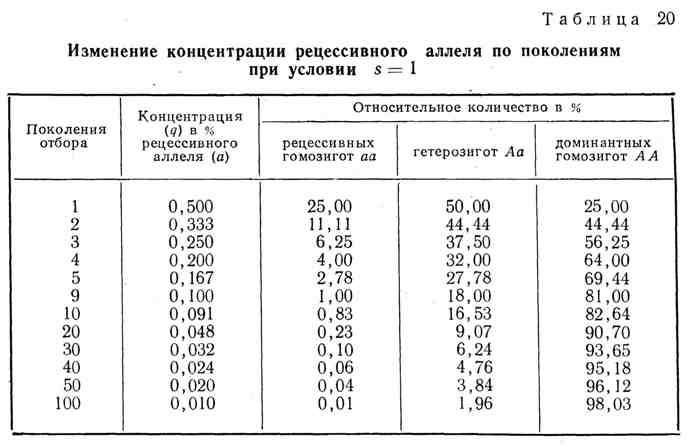
\includegraphics[width=0.80\textwidth]{img/1_7_0.png}
\end{center}

\section*{1.8}

\begin{center}
	\LARGE{\textbf{Что такое глобальное потепление?}}\\
\end{center}

Глобальное потепление это антропогенное повышение средней температуры климатической системы Земли за длительный промежуток времени. Климатической системой называют объединение атмосферы, гидросферы,криосферы, литосферы и биосферы. Многочисленные независимые наборы данных подтверждают, что десятилетие 2009-2018 годов было на 0,93 $\pm$ 0,07 $^\circ$C теплее доиндустриального периода (1850-1900). В настоящее время температура поверхности повышается примерно на 0,2 $^\circ$C в десятилетие. Климатическая модель прогнозирует, что в 21 веке средняя температура всей поверхности Земли может вырасти еще на 0,3-1,7  $^\circ$C при умеренном сценарии или даже на 2,6-4,8  $^\circ$C при экстремальном сценарии.

Последствия глобального потепления включают повышение уровня моря, региональные изменения осадков, учащение экстремальных погодных явлений, таких как аномальная жара, и расширение пустынь. Закисление океана также вызвано выбросами парниковых газов и обычно группируется с этими последствиями, даже если оно не обусловлено растущей температурой. Наибольшее повышение температуры поверхности наблюдается в Арктике, что способствовало таянию ледников, вечной мерзлоты и морского льда. В целом, повышение температуры приводит к увеличению количества осадков и снегопадов, но в некоторых регионах наоборот засухи и лесные пожары усилятся. Изменение климата угрожает снижением урожайности сельскохозяйственных культур, подрывает продовольственную безопасность, а повышение уровня моря может привести к затоплению прибрежной инфраструктуры и вынудить покинуть многие прибрежные города. Экологические последствия включают исчезновение или перемещение многих видов по мере изменения их экосистем, в первую очередь коралловых рифов, гор и Арктики.

\section*{1.9}

\begin{center}
	\LARGE{\textbf{Чему равна скорость звука в различных средах?}}\\
\end{center}

Скорость звука в жидкости или газе вычисояется по следующей формуле:
$$c = \sqrt{\frac{1}{\beta \rho}}$$

Для воздуха при нормальных условиях
$C_{\text{в}} = 331.46$ м/с

Для воды при нормальных условиях
$C_{\text{H2O}} = 1500$ м/с

Скорость звука в кристалле можно посчитать по формуле 
$$v=\sqrt{\frac{k}{m}}d$$
Где d - период кристаллической решетки, k - коэффициент квазиупругой силы, а m масса молекулы (атома).

\section*{1.10}

\begin{center}
	\LARGE{\textbf{Сколько тепла выделяется при стирании одного бита информации?}}\\
\end{center}

\textbf{Почему рассеивается энергия? Логическая необратимость и ее связь с дисспациями.}
 
Назовем устройство логически необратимым, если по сигналу на выходе нельзя однозначно определить сигнал на входе. Логическая необратимость предполагает физическую необратимость, которая приводит к диссипативным эффектам.

\subsection*{Пример}
Примером необратимой логической функции истинности может являться установление в единицу.
Покажем необратимость. Бинарное устройство представляет собой частицу в бистабильной потенциальной яме. Если бы мы могли перевести частицу из состояния ноль или единица в единицу без потерь энергии, то так как система консервативна, "обратив" время, мы получим систему, которая по-прежнему будет удволетворять уравнениям движения. В этой системе для одного начального условия результатом будут два состояния(ноль и единица), однако законы механики полностью детерминированы, и траектория определяется начальным положением и скоростью.

\subsection*{Энтропия}

Остается изучить связь между логической необратимостью и \textbf{энтропией}:
\begin{equation}
	S = k \ln W,
\end{equation}
где $k$ -- постоянная Больцмана, $W$ -- статистическая вероятность (число микросостояний, реализующее данное макросостояние системы).

При стирании число состояний уменьшается в 2 раза, то есть энтропия уменьшается на $k \ln 2$.
Энтропия замкнутой системы не может уменьшаться,следовательно она должна проявиться в виде эффекта нагревания, тогда выделится $E\succeq k T \ln 2$ \textbf{(Принцип Ландауэра).}

Ограничения, накладываемые принципом Ландауэра можно обойти путём реализации обратимых вычислений, при этом возрастают требования к объёму памяти и количеству вычислений.

\section*{2.3}
\begin{center}
	\LARGE{\textbf{Элементарные частицы и их свойства.}}\\
\end{center}
\begin{scriptsize}
\begin{center}
\begin{tabular}{cccccccc}
\hline
& Электрический & Цветной & Барионное& Спин & Магнитный  & Изоспин & Внутренняя\\
& заряд &заряд& число & & момент  && четность\\
Протон & +1 &"белый"& 1 &  1/2 & 1,41060679736(60)$\cdot10^{-26}$  & 1/2& 1\\
Нейтрон & 0 &"белый"& 1 &  1/2 & -9,6623651(23)$\cdot10^{-27}$ & -1/2& 1\\
\hline
& Электрический &Цветной& Барионное& Спин & Слабый & Изоспин& Четность\\
& заряд &заряд& число & & гиперзаряд && \\
Пион &$\pm1$ & "белый"&0&0&0, -2, -1&$\pm1$& -
\\
\hline
& Электрический &Цветной& Лептонное & Спин & Магнитный && Внутренняя   \\
& заряд &заряд& число & & момент && четность\\
Электрон & -1 &0 & 1 & 1/2 & -9,274009994(57)$\cdot10^{-24}$ && 1
\\
\hline
& Электрический &Цветной& Лептонное & Спин &&& \\
& заряд & заряд & число &&&&  \\
Мюон & -1 &0& 1 & 1/2 &&&
\\
\hline
& Электрический &Цветной& Лептонное & Спин & Кол-во спиновых   \\
& заряд &заряд& число & & состояний \\
$\tau$-лептон & -1 &0& 1 & 1/2 & 2
\\
\hline
& Электрический &Цветной& Лептонное & Спин & Слабый  \\
& заряд &заряд& число & & гиперзаряд \\
Нейтрино & 0 & 0 & 1 & 1/2 & -1
\\
\hline
& Электрический &Цветной& Барионное & Спин  \\
& заряд &заряд& число & \\
Кварк & кратен e/3 & r, g, b & 1/3 & 1/2 
\\
\hline
& Электрический & Цветной && Спин & Количество спиновых  \\
& заряд & заряд &&& состояний\\
W$^+$- базон & +1& 0&& 1&3\\
W$^-$- базон& -1 &0 &&1&3\\
Z -  базон&0 &0 && 1&3\\
\hline
& Электрический &Цветной&& Спин &Кол-во спиновых&& Внутренняя\\
& заряд &заряд&& & Состояний&& четность \\
Глюон& 0& $r\bar r, g\bar g, b\bar b, r\bar g, r\bar b, g\bar b$,&& 1& 2&& -
\\
\hline
&Эликтрический& Цветной&& Спин& Кол-во спиновых& Спиральность& Внутренняя\\
&заряд& заряд&&& состояний&&четность\\
Фотон &0& 0&& 1& 2& $\pm$1& -
\\
\hline
&Электрический& Цветной&& Спин&&& Четность\\
&заряд& заряд\\
Базон Хиггса &0& 0&& 0&&& +1\\
\hline
\end{tabular}
\end{center}
\end{scriptsize}

Электрический заряд - квантовое число, определяющее способность частиц принимать участие в электромагнитном взаимодействие.\\
Цветной заряд — квантовое число, приписываемое глюонам и кваркам, которые участвуют в сильном взаимодействии. Цветов три: «красный», «зелёный» и «синий», хотя эти названия не имеют никакого отношения к цветам, которые мы видим в повседневной жизни, также существуют три антицвета.\\
Спин — собственный момент импульса элементарных частиц. Спин измеряется в единицах $\hbar$ (постоянной Дирака) и равен $\hbar$J, где J — характерное для каждого сорта частиц целое или полуцелое положительное число — так называемое спиновое квантовое число, которое и приведено в таблице.\\
Изоспин — квантовое число, определяющая число зарядовых состояний адронов.\\
Магнитный момент — квантовое число, характеризующее магнитные свойства частицы. Измеряется в Дж/Тл.\\
Барионное число — квантовое число, определяющее количество барионов (элементарных частиц, состоящих из трёх кварков) в системе.\\
Лептонное число — разность числа лептонов (частиц с полуцелым спином, не участвующих в сильном взаимодействии) и антилептонов в данной системе.\\
Спиральность — квантовое число, используемое при описании элементарных частиц, движущихся со скоростью света или близкой к ней.

\section*{2.4}

\begin{center}
	\LARGE{\textbf{Хронология событий во Вселенной.}}\\
\end{center}

\begin{enumerate}
\item \textbf{Планковская эпоха}  $0 - 10^{-43}$ c

Момент, с которого началась физика. После Планковской эпохи гравитационное взаимодействие отделилось от отстальных.
\item \textbf{Эпоха великого объединения} $10^{-43} - 10^{-34}$ c

С момента начала ЭВО квантовые эффекты слабеют и вступают в силу законы ОТО.

\item \textbf{Эпоха раздувания} $10^{-36} - 10^{-32}$ c

В эту эпоху Вселенная всё ещё преимущественно заполнена излучением, начинают образовываться кварки, электроны и нейтрино.

\item \textbf{Эпоха электрослабых взаимодействий} $10^{-32} - 10^{-12}$ c

За счёт очень высоких энергий образуется ряд экзотических частиц, таких как бозон Хиггса и W-бозон, Z-бозон.

\item \textbf{Эпоха кварков} $10^{-12} - 10^{-6}$ c

Электромагнитное, гравитационное, сильное, слабое взаимодействия формируются в их современном состоянии.

\item \textbf{Эпоха адронов} $10^{-6} - 100$ c

Кварк-глюонная плазма охлаждается, и кварки начинают группироваться в адроны, включая, например, протоны и нейтроны.

\item Эпоха лептонов 100 c - 3 мин

В ходе адронной эпохи большая часть адронов и антиадронов аннигилируют (взаимоуничножаются) друг с другом и оставляют пары лептонов и антилептонов преобладающей массой во Вселенной. Лептоны и антилептоны, в свою очередь аннигилируют друг с другом и во Вселенной остаётся лишь небольшой остаток лептонов.

\item \textbf{Протонная эпоха} 3 мин - 380 000 лет

материя охладилась достаточно для образования стабильных нуклонов и начался процесс первичного нуклеосинтеза. за это время образовался первичный состав звёздного вещества: около 25 $\%$ гелия-4, 1 $\%$ дейтерия, следы более тяжёлых элементов до бора, остальное — водород.

\item \textbf{Темные века} 380 000 лет - 550 млн лет

Вещество начинает доминировать над излучением (70 000 лет), что приводит к изменению режима расширения Вселенной. В конце эпохи (380 000 лет) происходит рекомбинация водорода и Вселенная становится прозрачной для фотонов теплового излучения.

\item \textbf{Реонизация} 550 млн лет - 800 млн лет

Образуются первые звёзды, галактики, квазары, скопления и сверхскопления галактик. Реионизация водорода светом звёзд и квазаров.

\item \textbf{Эра вещества} 800 млн лет - сейчас

Образование межзвёздного облака, давшего начало Солнечной системе. Образование Земли и других планет нашей Солнечной системы, затвердевание пород.
\end{enumerate}

\section*{2.5}

\begin{center}
	\LARGE{\textbf{Как проявляются законы Кеплера в атоме водорода?}}\\
\end{center}

Задача Кеплера, это когда:\\
$\mathbf {F} ={\frac {k}{r^{2}}}\mathbf {\hat {r}}$\\
$V(r)={\frac {k}{r}}$, где $V(r)$ - потенциальная энергия\\
Нетрудно заметить, что в модели атома Бора для водорода эти условия выполняются.\\
Таким образом, можно применить к движению электрона в атоме водорода и получить:\\
1. электрон движется по эллипсу(окружности)(1 закон Кеплера)\\
2. за равное время заметает равные секторальные площади(2 закон Кеплера)\\
3. 3 закон Кеплера\\
А исходя из этих законов можно посчитать период обращения электрона на разных энергетических уровнях, различные параметры траектории и т.д.\\

\section*{2.6}

\begin{center}
	\LARGE{\textbf{Чему "равны" интегралы?}}\\
\end{center}

\begin{equation}
y = \int_0^\infty \frac{e^{-z}}{(1 + x z)}\;\mathrm{d}z = \frac{e^{1/x} \Gamma \left(0,\frac{1}{x}\right)}{x},\Im(x)\neq 0\lor \Re(x)\geq 0
\end{equation}
Как видно из графиков максимальное значение интеграла $\approx$ 2 и достигается при $x\approx 0.001354$\\
При $x<0.001354$ значение интеграла 0\\
При $x>0.001354$ значение будет "осциллировать" с убывающей амплитудой, а "среднее" будет просто убывать, стремясь к 0 
\begin{figure}[h]
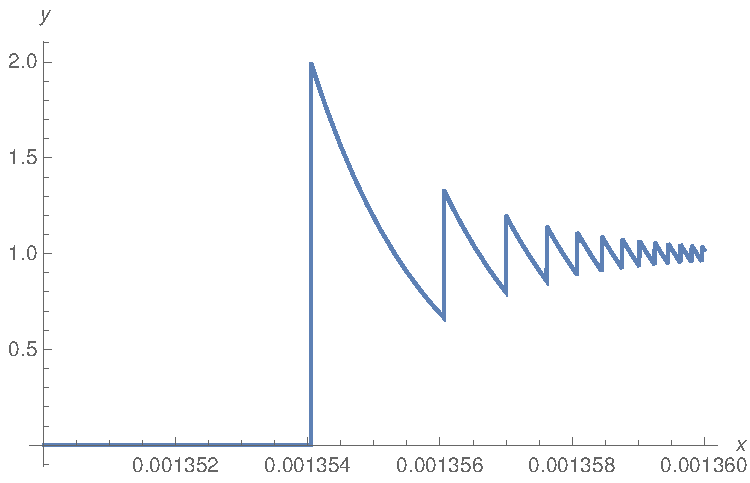
\includegraphics{gr1}
\end{figure}

\begin{figure}[h]
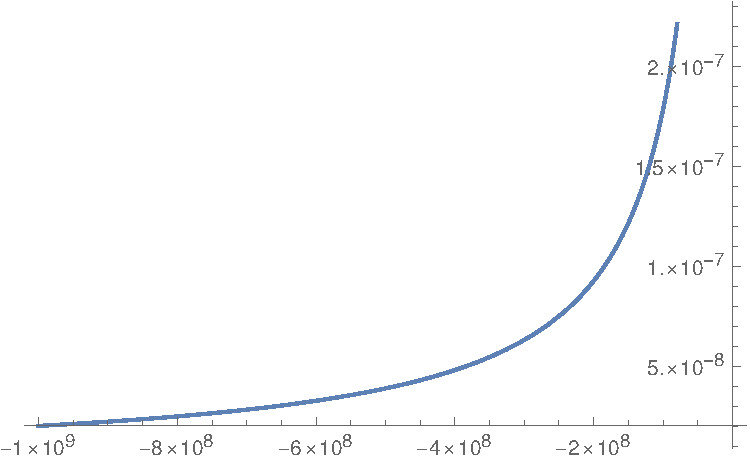
\includegraphics{gr2}
\end{figure}

\begin{equation}
y_2 = \int_{-\infty }^{\infty } e^{-x z^4-\frac{z^2}{2}} \, dz = \frac{e^{\frac{1}{32 x}} K_{\frac{1}{4}}\left(\frac{1}{32 x}\right)}{2 \sqrt{2} \sqrt{x}},\Re(x)>0
\end{equation} 

Как видно из графиков максимальное значение интеграла $\approx$ 5.3 при $x\approx 0.0000421$\\
При $x<0.0000421$ значения максимума значение интеграла равно 0\\
При $x>0.0000421$ значения максимума значение интеграла начинает "осциллировать", а "среднее" будет убывать, стремясь к 0

\begin{center}
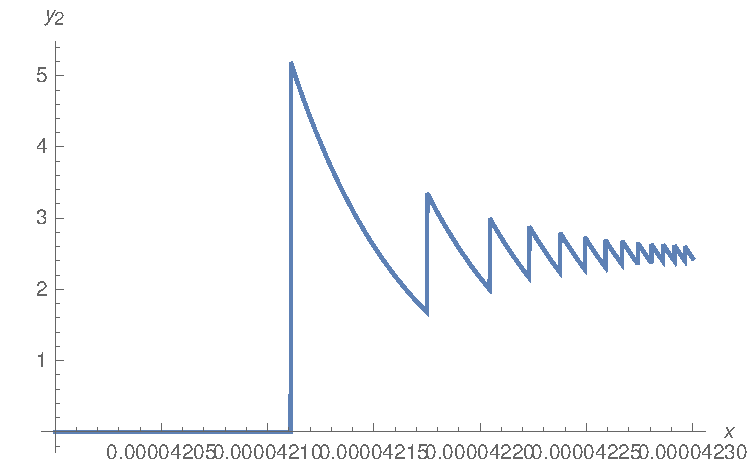
\includegraphics{gr4}
\end{center}

\begin{center}
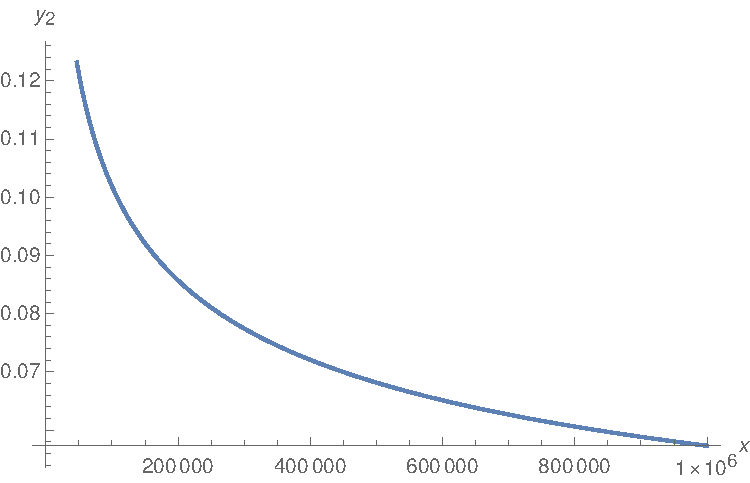
\includegraphics{gr5}
\end{center}

\section*{2.7}

\begin{center}
	\LARGE{\textbf{Отличия ДНК от РНК.}}\\
\end{center}

\begin{enumerate}
\item Мономерная единица ДНК --- дезоксирибонуклеотид, РНК --- рибонуклеотид.
\newline
Рибонуклеотид образован рибозой, азотистым основанием и остатком фосфорной кислоты. Рибоза --- пятиуглеродный моносахарид. Рибоза, входящая в состав биологических структур, обладает свойством хиральной чистоты: молекулы РНК построены исключительно на «правой» рибозе.
\newline
Дезоксирибонуклеотид образован дезоксирибозой, азотистым основанием и остатком фосфорной кислоты. Дезоксирибоза --- производное рибозы, где гидроксильная группа у второго атома углерода замещена водородом с потерей атома кислорода (дезокси --- отсутствие атома кислорода).
\newline
Таким образом, у рибозы есть дополнительная, по сравнению с дезоксирибозой, гидроксильная группа. Эта группа увеличивает вероятность гидролиза молекулы, то есть уменьшает стабильность молекулы РНК.

\item Азотистые основания в молекуле ДНК – тимин, аденин, цитозин, гуанин; в РНК же комплементарный аденину нуклеотид --- не тимин, а урацил --- неметилированная форма тимина.

\item Отличаются функции молекул. ДНК является матрицей для транскрипции, она хранит генетическую информацию. Основная функция молекулы ДНК в клетках --- точное сохранение информации о строении белков и РНК. РНК же участвует в синтезе белка: информационная РНК (иРНК) синтезируется на основе ДНК в ходе транскрипции, после чего, в свою очередь, используется в ходе трансляции как матрица для синтеза белков; транспортная РНК (тРНК) отвечает за доставку аминокислот к рибосомам; рибосомная РНК является составляющей рибосом, она считывает информацию с иРНК и катализирует образование пептидных связей между присоединёнными к тРНК аминокислотами. У молекул РНК есть и другие функции: например, малые ядерные РНК принимают участие в сплайсинге эукариотических матричных РНК и других процессах. 
\newline
Есть исключение: РНК является составной частью геномов большинства вирусов, у которых она выполняет ту же функцию, что и ДНК у высших организмов.

\item ДНК существует в форме двойной спирали, состоящей из двух отдельных молекул. Молекулы РНК, в среднем, гораздо короче и преимущественно одноцепочечные. Структурный анализ биологически активных молекул РНК, включая тРНК, рРНК и другие молекулы, которые не кодируют белков, показал, что они состоят не из одной длинной спирали, а из многочисленных коротких спиралей, расположенных близко друг к другу и образующих нечто, похожее на третичную структуру белка. В результате этого РНК может катализировать химические реакции, например, пептидил-трансферазный центр рибосомы, участвующий в образовании пептидной связи белков, полностью состоит из РНК.
\end{enumerate}

\section*{2.8}

\begin{center}
	\LARGE{\textbf{Параметры, характеризующие глобальное потепление.}}\\
\end{center}

\begin{enumerate}

\item \textbf{Средняя приповерхностная температура воздуха}
\newline
За период 1901-2012 гг. она выросла на $(0,89 \pm 0,20) \degree C$. Данные о динамике средней годовой температуры на планете можно найти, например, на сайте Университета Восточной Англии (рис. 1), на сайте американского Национального управления океанических и атмосферных исследований и на сайте Института космических исследований Годдарда, входящего в NASA. Наибольшее потепление произошло за последние 35 лет, причём пять самых тёплых лет за всю историю наблюдений имели место с 2010 года. 2016 год был самым тёплым за всю историю наблюдений, причём восемь из 12 месяцев, составляющих год - с января по сентябрь, за исключением июня - были самыми теплыми за всю историю наблюдений за эти месяцы.

\begin{figure}[h!]
\center{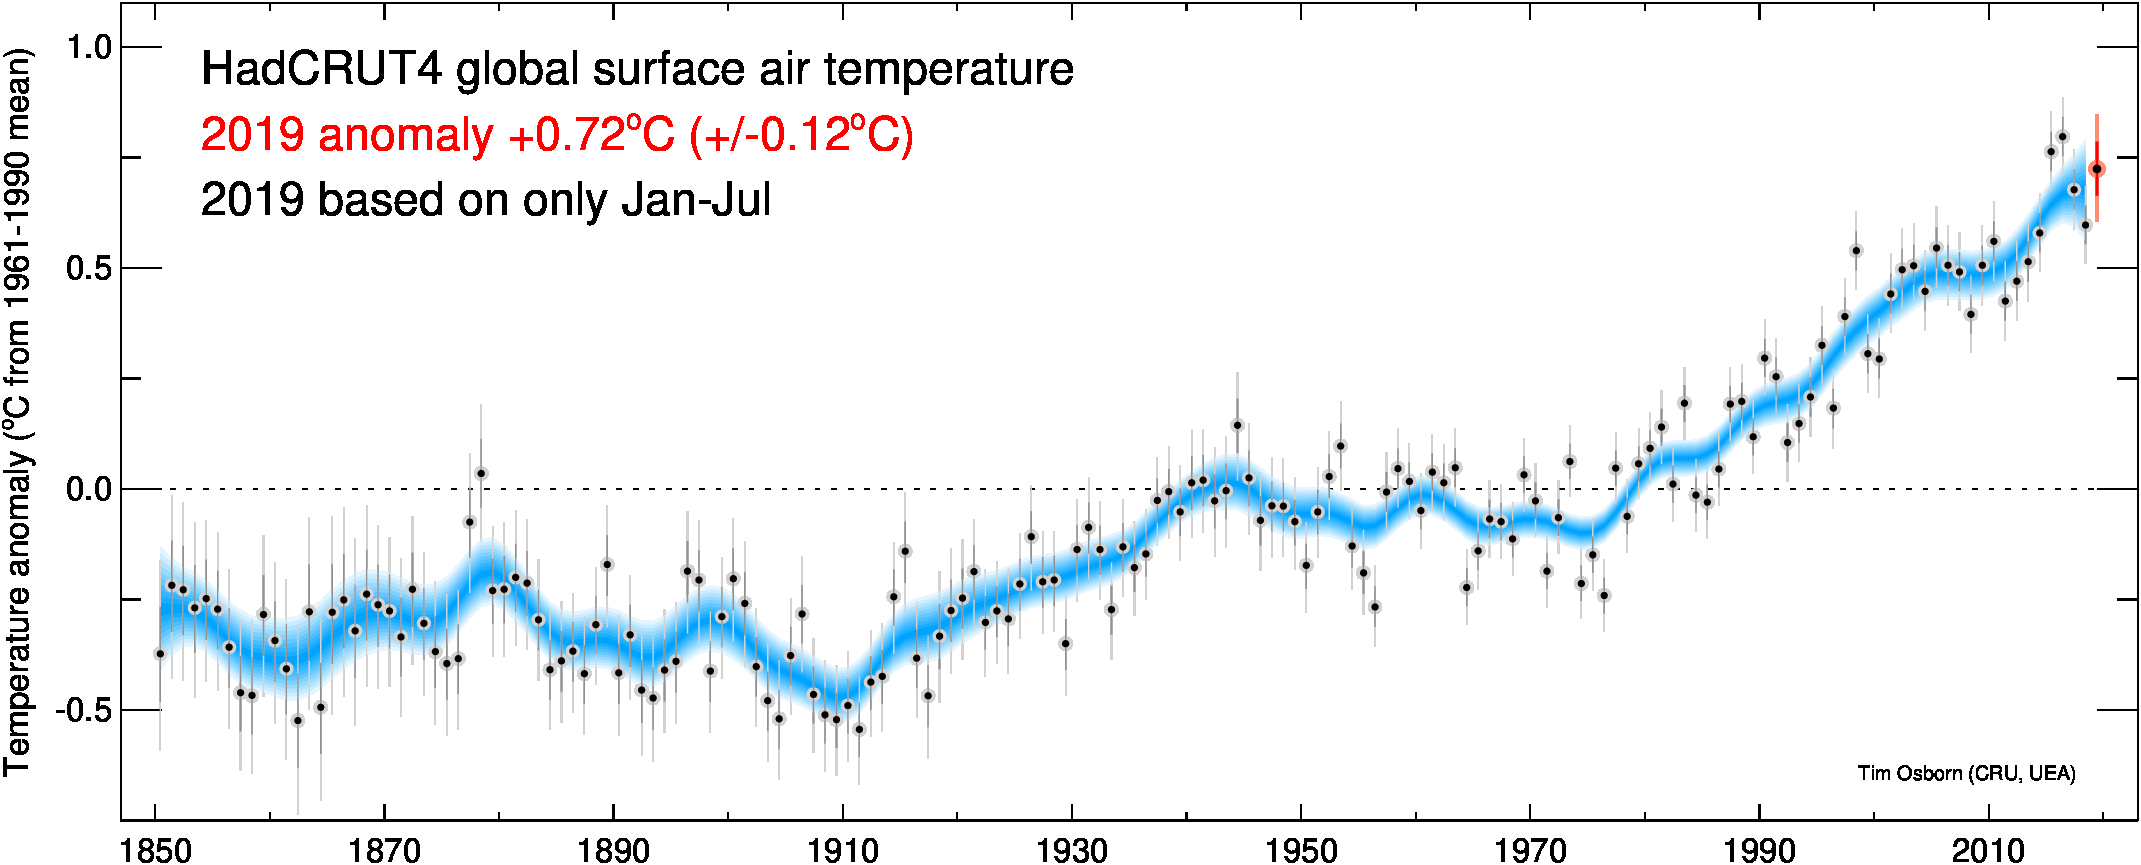
\includegraphics[scale=0.21]{average_temperature}}
\caption{Зависимость разности глобальной средней приповерхностной температуры воздуха и её среднего значения в период 1961-1990 гг. от времени}
\end{figure}

\item \textbf{Рост теплосодержания океана}
\newline
Океаны абсорбируют большое количество выделяющегося тепла. С 1969 г. температура верхних 700 м океана выросла более чем на $0,2 \degree C$ (Levitus et al, 2017).

\item \textbf{Рост уровня мирового океана} (вызванный термическим расширением воды при нагревании и таянием ледяного покрова)
\newline
Согласно данным Института космических исследований Годдарда (рис. 2), с 1993 года уровень мирового океана вырос на $(95 \pm 4) \; \text{мм}$. Текущая скорость увеличения уровня --- $(3,3 \pm 0,4) \; \text{мм}/\text{год}$. По данным австралийского Государственного объединения научных и прикладных исследований (рис. 3), с 1880 г. уровень океана вырос примерно на 230 мм.

\begin{figure}[h!]
\center{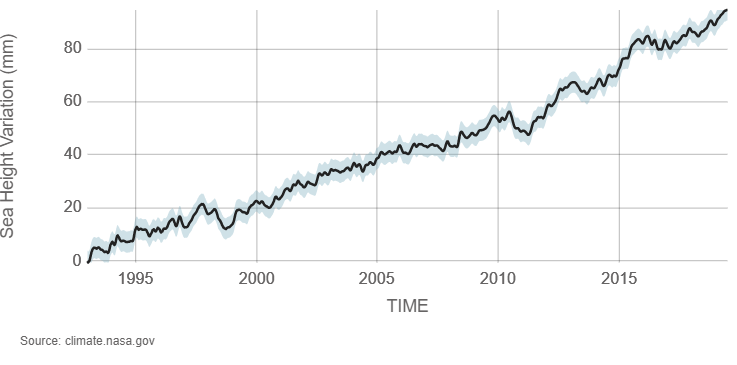
\includegraphics[scale=0.4]{SeaLevel}}
\caption{Зависимость изменения уровня мирового океана по сравнению с 1993 г. от времени}
\end{figure}

\begin{figure}[h!]
\center{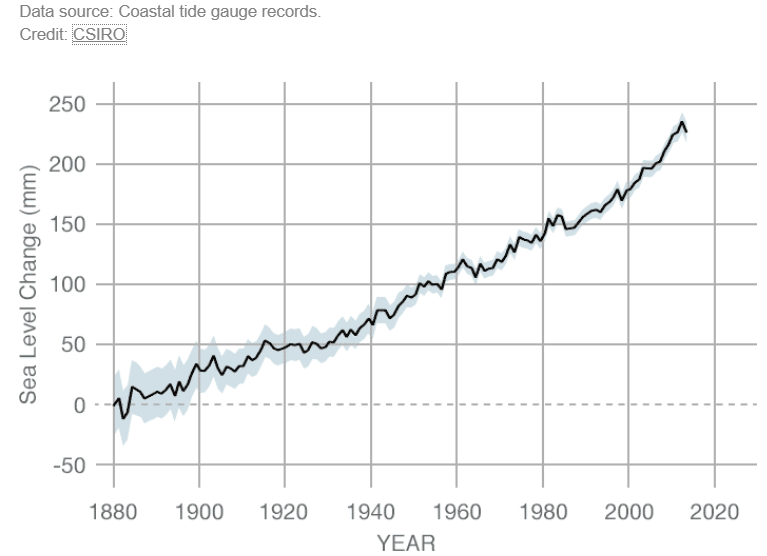
\includegraphics[scale=0.5]{SeaLevel1}}
\caption{Зависимость изменения уровня мирового океана по сравнению с 1880 г. от времени}
\end{figure}

\item \textbf{Уменьшение площади арктического морского льда}
\newline
Годовой минимум площади арктического морского льда достигается в сентябре. По данным NASA (рис. 4), в 1980 г. площадь сентябрьского льда составляла $7,67 \; \text{млн} \; \text{км}^{2}$, в 2019 г. --- $4,32 \; \text{млн} \; \text{км}^{2}$; 

\begin{figure}[h!]
\center{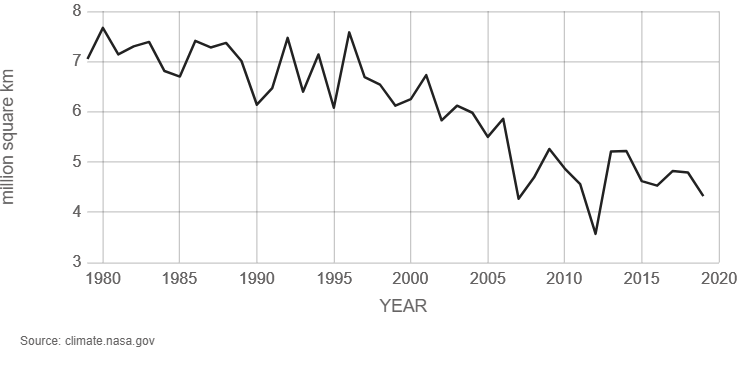
\includegraphics[scale=0.4]{SeaIce}}
\caption{Зависимость площади сентябрьского морского льда в Арктике от года}
\end{figure}

\item \textbf{Уменьшение ледяных покровов}
\newline
По данным NASA, Гренландия в среднем теряла 286 млрд тонн льда в год в период с 1993 по 2016 г., в то время как Антарктика в этот же самый период теряла в среднем 127 млрд тонн льда в год. При этом внутренние области Восточной Антарктики наращивают лёд, однако в целом она теряет его с ускоряющимся темпом.

\item \textbf{Увеличение концентрации углекислого газа в атмосфере}
Согласно данным Национального управления океанических и атмосферных исследований (рис. 5), в октябре 2019 г. концентрация углекислого газа в атмосфере составляла 412 ppm. Это самое большое значение величины как минимум за последние 400 тысяч лет (рис. 5).

\begin{figure}[h!]
\center{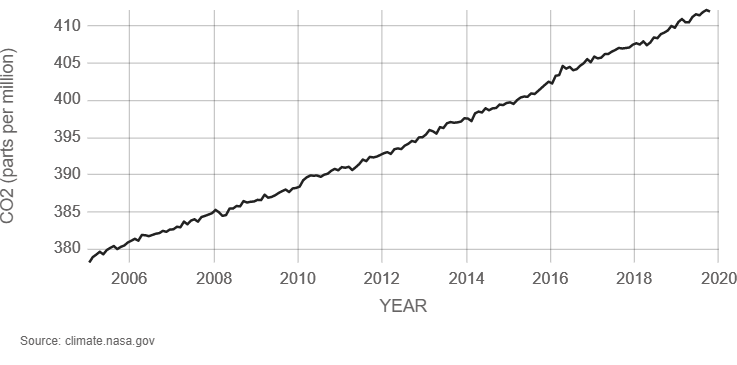
\includegraphics[scale=0.4]{CO2}}
\caption{Зависимость концентрации углекислого газа в атмосфере от времени с 2006 г.}
\end{figure}

\begin{figure}[h!]
\center{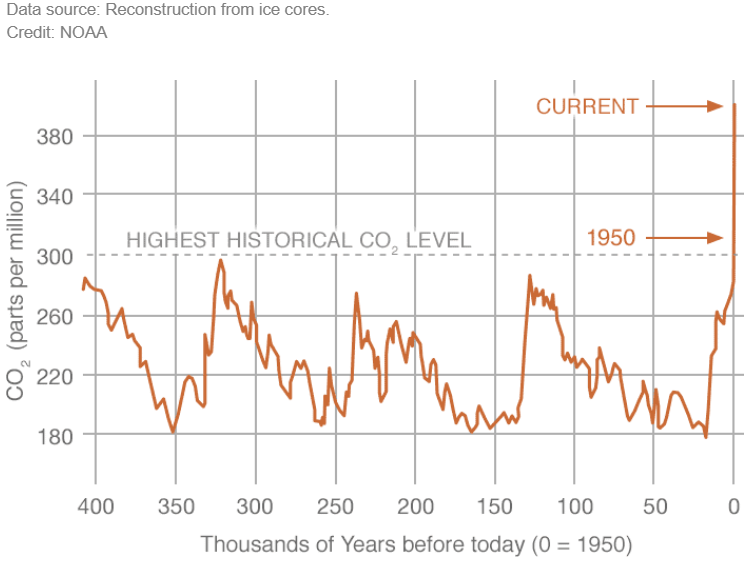
\includegraphics[scale=0.5]{CO2_long}}
\caption{Зависимость концентрации углекислого газа в атмосфере от времени за последние 400 тысяч лет}
\end{figure}

\end{enumerate}

В настоящее время подавляющее большинство специалистов-климатологов считают, что основная причина быстрого изменения климата --- деятельность человека (Cook et al, 2013). Вот некоторые факты, которые позволяют проследить эту связь:
\begin{itemize}
\item В атмосфере растёт количество углекислого газа --- сейчас оно почти в полтора раза превышает максимумы за последние 400 тысяч лет. 
\item Сжигание ископаемых топлив является основной причиной антропогенной эмиссии $CO_{2}$. В северном полушарии, где сжигается большая часть топлива, концентрация $CO_{2}$ выше, чем в южном.
\item Концентрация кислорода падает так, как было бы, если бы он полностью уходил на сжигание топлива.
\item В атмосферном углекислом газе становится относительно меньше изотопов углерода-14 и углерода-13, которых нет в нефти и угле.
\item $CO_{2}$ является парниковым газом.
\item Глобальная температура быстро растёт. При этом интенсивность солнечного излучения в последние 35 лет падает. Это и другие доказательства опровергают возможность связи нынешнего увеличения температуры с солнечной активностью, о которой говорят некоторые противники теории антропогенного изменения климата. Кроме того, некоторые учёные предполагают, что это уменьшение солнечной активности может быть началом "большого минимума" наподобие маундеровского. Однако в ряде статей (см. сноску 2, climate.nasa.gov/blog/2910/what-is-the-suns-role-in-climate-change/) делается вывод, что это может в лучшем случае на несколько лет замедлить вызванное человеком потепление.
\end{itemize}

Некоторые скептики говорят о том, что нынешнее потепление --- естественное явление, подобное случавшимся ранее в истории Земли. Сторонники теории антропогенной природы потепления отвечают следующим образом: естественные климатические изменения в прошлом подтверждают, что климат чувствителен к энергетическому дисбалансу. Если планета аккумулирует тепло, глобальные температуры будут расти. В настоящее время $CO_{2}$ вызывает энергетический дисбаланс благодаря парниковому эффекту. Изменения климата в прошлом на самом деле подтверждают чувствительность климата к $CO_{2}$, а увеличение количества $CO_{2}$ вызвано деятельностью человека.
\newline

\section*{2.9}
\begin{center}
	\LARGE{\textbf{Чему равны для идеального газа коэффициенты диффузии теплопроводности и вязкости?}}
\end{center}	
Коэффициент диффузии для идеального газа: \[ D=\frac{1}{3}<\lambda><v>=\frac{1}{3}\frac{1}{\sqrt{2} \pi d^2 n} \sqrt{\frac{8 R T}{\pi \mu}},\] где <$\lambda$> - средняя длина свободного пробега молекул, d - диаметр молекул, n - концентрация молекул; <v> - средняя арифметическая скорость молекул, R-газовая постоянная, $\mu$ - молярная масса, T - температура.
\\Коэффициент теплопроводности для идеального газа: \[ \chi=\rho C_{v} D,\] где $C_{v}$ - удельная изохорическая теплоёмкость газа $(C_{v}=\frac{i}{2}\frac{R}{M})$, $\rho$ - плотность газа.
\\Коэффициент вязкости для идеального газа: \[\nu=\rho D,\].

\section*{2.10}
\begin{center}
	\LARGE{\textbf{Спектр и мощность излучения черного тела в $d + 1$ измерении.}}
\end{center}
Излучение абсолютно черного тела в $(n|n > 1)$ пространстве -- известная задача, решение которой человечество уже нашло. Из статьи 2005 года $"$The blackbody radiation in a D-dimensional universes (dx.doi.org/10.1590/S1806-11172005000400007)$"$ видно, что спектр тела в $d+1$ мерном пространстве равен:
\begin{equation*}
	\rho_T(\nu) = 2 \left( \frac{\sqrt{\pi}}{c} \right) ^{d + 1} \frac{d}{\Gamma \left( \frac{d + 1}{2} \right)}\cdot\frac{h\nu^{d + 1}}{exp(h\nu / k_B T) - 1},
\end{equation*}
а энергия излучения на единицу площади равна:
\begin{equation*}
	\sigma_d T^{d + 2},
\end{equation*}
где $\sigma_d$ -- постоянная Стефана — Больцмана $d + 1$ мерного пространства, равная:
\begin{equation*}
	\sigma_d = \left( \frac{2}{c} \right) (\sqrt{\pi})^{d - 1} \frac{k_B^{d+2}}{h^{d + 1}} d (d + 1) \Gamma \left( \frac{D}{2} \right) \zeta(d + 2).
\end{equation*}

\section*{3.3}
\begin{center}
	\LARGE{\textbf{Уравнения движения и лагранжиан электромагнитного поля.}}
\end{center}

Свойства поля характеризуются 4-потенциалом $A_i$ в кажоый точке пространства-времени. Он определен с точностью до $\frac{\delta f}{\delta x^i}$, где f -- произвольная функйия от координат и времени. Привычные нам величины -- векторы электрического и магнитных полей выражаются через тензор электромагнитного поля:
\begin{equation*}
	F_{\mu \nu} = \begin{pmatrix}
		0 & E_x & E_y & E_z \\
		-E_x & 0 & -B_z & B_y \\
		-E_y & B_z & 0 & -B_x \\
		-E_z & -B_y & B_x & 0
	\end{pmatrix},
\end{equation*}
где тензор электромагнитного поля определяется через 4-потенциал, как:
\begin{equation*}
	\mathrm{F}_{\mu \nu} = \frac{\delta A_\nu}{\delta x^\mu} - \frac{\delta A_\mu}{\delta x^\nu}.
\end{equation*}
Лагранжиан электромагнитного поля равен:
\begin{equation*}
	L_{em} = -\frac{1}{4}F_{\mu \nu}F_{\mu \nu} + \frac{1}{c}j_\mu A_\mu.
\end{equation*}
Уравнения движения электромагнитного поля (которые, кстати, выводятся из Лагранжиана) известны под названием "уравнения Максвелла", и представляют из себя систему из 4 уравнений, описывающих эволюцию электромагнитного поля со временем (в си):
\begin{equation*}
	\begin{cases}
		\nabla \cdot \mathbf{E} = \frac {\rho} {\varepsilon_0},\\
		\nabla \cdot \mathbf{B} = 0,\\
		\nabla \times \mathbf{E} = -\frac{\partial \mathbf{B}} {\partial t},\\
		\nabla \times \mathbf{B} = \mu_0\left(\mathbf{J} + \varepsilon_0 \frac{\partial \mathbf{E}} {\partial t} \right).
	\end{cases}
\end{equation*}

\section*{3.4}

\begin{center}
	\LARGE{\textbf{В чем состоит, зачем нужна и в чем проявляется космологическая инфляция.}}\\
\end{center}

Инфляционные модели рассматриваются на стр. 233-250 Космология, URSS Москва, 2 изд., 2018 (С.Вайнберг) .

Суть:
Идея инфляции предполагает наличие эпохи экспоненциального роста масштабного фактора $а(t)$, предшествующей эре доминирования излучения ($a(t)\sim\sqrt{t}$).

Необходимость:
Алан Гут обнаружил, что наличие инфляционного периода способно разрешить ряд проблем космологии
а)Плоскостность (необходимость объяснить, как Вселенной на ранних стадиях удавалось поддерживать околонулевую кривизну)
б)Горизонты (в период доминирования вещества или излучения никакое физическое воздействие не могло сгладить начальные неоднородности, а в период инфляции наблюдаемая нами часть Вселенной могла занимать крошечный объём и с тех пор дать всему внутри этого объёма распределиться однородно)
в)Монополи (классическая модель большого взрыва предсказывала в наблюдаемой Вселенной число монополей, значительно расходящееся с полученными данными)

Проявления:
Помимо согласования наблюдаемых данных и теории касательно указанных выше величин, инфляционные модели смогли предсказать некоторые свойства флуктуаций реликтового излучения и крупномасштабной структуры Вселенной.
Это делает идею инфляции ещё более правдоподобной.

\section*{3.5}

\begin{center}
	\LARGE{\textbf{Симметрии и законы сохранения при движении частицы в кулоновском поле.}}\\
\end{center}

В кулоновском поле у частицы сохраняется энергия, момент имупульса и вектор Рунге-Ленца. 

Энегрия: 

\begin{equation*}
E = \frac{M}{2} \dot{r}^2 + \frac{L^2}{2Mr^2} - \frac{k}{r} = const
\end{equation*}
Где $\mathbf {L} = [\mathbf r \times \mathbf P ]$ - момент импульса частицы, $M$ - ее приведенная масса, $U = - \frac{k}{r}$ - потенциальная энергия, а $r$ - радиус вектор из начала координат. 

Разберемся с моментом импульса тела, т.к. момент силы, действующей на частицу нулевой, то:
\begin{equation*}
\mathbf {M} = [\mathbf r \times \mathbf F ] = 0 ; \quad  [\mathbf r \times \frac{d \mathbf P}{dt} ] = 0
\end{equation*}
Следовательно момент импульса $L$:
\begin{equation*}
\frac{d}{dt} [\mathbf r \times \mathbf P ] = [\mathbf r \times \frac{d \mathbf P}{dt} ] +  [\frac{d\mathbf r}{dt} \times \mathbf P] = [\mathbf r \times \frac{d \mathbf P}{dt} ] = 0
\end{equation*}
Т.е. $\frac{d\mathbf L}{dt} = 0$, значит $L = [\mathbf r \times \mathbf P ]= const$

Определим вектор Рунге-Ленца, как:
\begin{equation*}
\mathbf A = [\mathbf P \times \mathbf L] - Mk\widehat{\mathbf r}
\end{equation*}
Данный вектор также сохраняется в кулоновском поле:
\begin{equation*}
\mathbf F =\frac{d \mathbf P}{dt} = f(r)\frac{\mathbf r}{|r|} = f(r)\widehat{\mathbf r}
\end{equation*}
Т.к. $L = const$
\begin{equation*}
\frac{d}{dt} [\mathbf P \times \mathbf L ] = \frac{d \mathbf P}{dt} \times \mathbf L =  f(r)\widehat{\mathbf r} \times \left(\mathbf r \times M \frac{d\mathbf r}{dt} \right) =  f(r)\frac{M}{r}\left[ \mathbf r\left(\mathbf r \frac{d\mathbf r}{dt}\right) - r^2\frac{d\mathbf r}{dt} \right]
\end{equation*}
Откуда получаем:
\begin{equation*}
\frac{d}{dt} [\mathbf P \times \mathbf L ] = -M f(r) r^2 \left[\frac{1}{r}\frac{d\mathbf r}{dt} - \frac{\mathbf r}{r^2}\frac{dr}{dt}  \right]
\end{equation*}
При $f(r) = -\frac{k}{r^2}$, последнее выражение равно:
\begin{equation*}
\frac{d}{dt} [\mathbf P \times \mathbf L ] = Mk\frac{d}{dt}\left( \frac{\mathbf r}{r}\right) = \frac{d}{dt}(Mk\widehat{\mathbf r})
\end{equation*}
Тогда изменение вектора:
\begin{equation*}
\frac{d}{dt}\mathbf A = \frac{d}{dt} [\mathbf P \times \mathbf L ] - \frac{d}{dt}(Mk\widehat{\mathbf r}) = 0
\end{equation*}
Отсюда получаем, что в кулоновском поле существует однородность времени, изотропность пространства, а также некоторая симметрия вектора Рунге-Ленца

\section*{3.6}

\begin{center}
	\LARGE{\textbf{Когда у уравнений $\bm{a_3x^3 + a_2x^2 + a_1x + a_0 = 0}$ и $\bm{b_2x^2 + b_1x + b_0 = 0}$ есть общее решение?}}\\
\end{center}

Многочлены в условии обозначим как $a(x)$ и $b(x)$.
Общие корни двух многочленов это корни их наибольшего общего делителя, поэтому у данных многочленов будет общий корень тогда и только тогда, когда будет корень у их НОДа. Для многочленов третьей и второй степени с данными коэфициентами НОД может быть быстро найден алгоритмом Эвклида, поиск потребует не более двух делений в столбик. В нашем случае остаток от деления первого многочлена на второй (в предположении $b_2\neq0$) равен 
$$
\left(a_1+a_3\frac{b_1^{2}}{b_2^{2}}-a_3\frac{b_0}{b_2}-a_2\frac{b_1}{b_2}\right) x + \left(a_0+a_3\frac{b_0 b_1}{b_2^{2}}-a_2\frac{b_0}{b_2}\right) = c_1 x + c_0 = c(x)
$$
Если $c(x) = 0$, то общий корень есть тогда и только тогда, когда у $b(x)$ вообще есть корень. Если $c_1 = 0$, но $c_0 \neq 0$, то общего корня нет. В противном случае корень есть тогда и только тогда, когда 
$$(b(x), c(x))=0\Leftrightarrow b\left(-\frac{c_0}{c_1}\right)=0\Leftrightarrow b_2\frac{c_0^{2}}{c_1^{2}}-b_1\frac{c_0}{c_1}+b_0=0.$$

\section*{3.7}

\begin{center}
	\LARGE{\textbf{Зависимость высоты прыжка от массы тела.}}\\
\end{center}

Определим вклад сопротивления воздуха в зависимость высоты прыжка от массы тела. Для этого рассмотрим вертикальный прыжок человека. По 2-му закону Ньютона относительно вертикальной оси $Ox$, направленной вверх: $ma_x(t) = -mg - kv_x^{\alpha}(t)$, где $\alpha = {1; 2}$ в зависимости от вида обтекания. Тогда нам нужно сравнить слагаемые $-mg$ и $-kv^{\alpha}$. Для этого возьмём предельную скорость падения человека, равную $v_\text{пр} \approx 60 \text{м}/\text{с}$ (измеренная предельная скорость парашютиста), тогда по 2-му закону Ньютона предельная сила сопротивления $F_\text{пр}$ равна по модулю силе $mg$. Взяв $v_0 \approx 3 \text{м}/\text{с}$ (можно оценить по собственному прыжку), найдём отношение максимальной силы сопротивления при данном прыжке $F_0$ к предельной:
\\
в случае турбулентного обтекания $\frac{F_0}{mg} = \frac{F_0}{F_{пр}} = \frac{k v_0^2}{k v_{пр}^2} = (\frac{v_0}{v_{пр}})^2 \approx \frac{1}{400}$;
\\
в случае ламинарного обтекания $\frac{F_0}{mg} = \frac{F_0}{F_{пр}} = \frac{k v_0}{k v_{пр}} = \frac{v_0}{v_{пр}} \approx \frac{1}{20}$.
\\
\smallskip
Можем видеть, что при любом обтекании даже максимальная сила сопротивления мала по сравнению с силой тяжести, и ей можно пренебречь.
\\
Стоит отметить, что для животных, способных прыгать с большой начальной скоростью (например, небольших насекомых) сила сопротивления может играть значительную роль.

\subsection*{Размеры тела}

Примем за $l$ характерный размер тела. Очевидно, его масса пропорциональна кубу размера: $m \sim l^3$. Сила $F$, которую способны создать мышцы тела, пропорциональна давлению $p$, возникающему вследствие веса тела, и площади сечения мышц $S$. Давление имеет верхний предел, поскольку начиная с некоторого значения массы тела кости и мышцы не выдержат нагрузки, поэтому можем считать давление постоянным для любой массы тела. Площадь $S$ же пропорциональна квадрату размера: $S \sim l^2$, отсюда $F \sim l^2$. Тогда работа, совершаемая мышцами при прыжке и пропорциональная $Fl$ (мышцы "проходят" большее расстояние при большем размере), будет так же, как и масса, пропорциональна кубу размера. Отсюда можно сделать вывод, что начальная кинетическая энергия тела на единицу массы, т.е. $v_0^2/2$, не зависит от размера. Как следствие, $v_0$ не зависит от размеров тела, так же как и высота прыжка.
\\
Данное рассуждение справедливо, если для людей верны приведенные пропорциональности. Если человек, например, обладает излишней массой, то начальная скорость прыжка будет все же меньше, нежели у человека такого же роста с нормальной массой тела. Как следствие, такой человек сможет прыгнуть не так высоко.

\section*{3.8}

\begin{center}
	\LARGE{\textbf{В чём состоит (утверждает) Общая теория относительности?}}\\
\end{center}

\subsection*{Введение}

	Создание специальной теории относительности в значительной мере изменило вид классической механики. Однако, в ней постулат относительности всё ещё ограничивается необходимостью выбора исключительного класса инерциальных систем отсчёта, двигающихся друг относительно друга равномерно и прямолинейно. Таким образом, становится вполне понятно, что общековариантные уравнения должны быть лишены этого ограничения, т. е. в общей теории должна быть возможность произвольного выбора координат.

	Так как в гравитационных полях пробные тела вне зависимости от их массы двигаются одинаковым образом, то вполне логично рассматривать такое движение как простое движение вдоль геодезических линий в криволинейном пространстве. 

	Общая теория относительности позволяет описать данные эффекты, будучи записанной при этом с помощью общековариантных уравнений, что решает вышпоставленные проблемы. 

\subsection*{Движение в гравитационном поле}

	Свойства пространства задаются метрическим тензором $ g_{ij} $ . Если тензор $ g_{ij} $
	получен в результате решения полевых уравнений, то уравнения движения частицы определяются варьированием действия для частицы. 

	\begin{align*}
		\delta S & = -mc \delta \int ds = 0 \\
	\end{align*}

	Из чего получаем уравнения движения:

	\begin{align*}
		D & u^i = 0 \\
		& или      \\
		\frac{d^2 x^i}{ds^2} + & \Gamma_{jk}^i \frac{dx^j}{ds} \frac{dx^k}{ds} = 0 \\
	\end{align*}

	где D - ковариантный диффиренциал, а $ \Gamma_{jk}^i $ - символ Кристоффеля: 

	\begin{align*}
		\Gamma_{jk}^i = \frac{1}{2} g^{im} & ( \partial_{j} g_{km} + \partial_{k} g_{jm} - \partial_{m} g_{jk} ) \\
	\end{align*}

	Решая их, можно получить уравнения движения частицы

\subsection*{Уравнения поля}	
	
	Для получения уравнений поля следует с начала определить тензор кривизны пространства (тензор Римана). Рассмотрим изменение вектора $ A_k $ при параллельном переносе его вдоль бесконечно малого контура:

	\begin{align*}
		\Delta A_k = \oint \delta A_k = \oint \Gamma_{kl}^i A_i dx^l 
		= \frac{1}{2} [ & \partial_l (\Gamma_{km}^i A_i) - \partial_m (\Gamma_{kl}^i A_i)] \Delta S^{lm} = \\
		= \frac{1}{2} [   \partial_l (\Gamma_{km}^i) A_i - \partial_m (\Gamma_{kl}^i) A_i + & (\Gamma_{km}^i) \partial_l A_i - (\Gamma_{kl}^i) \partial_m A_i ] \Delta S^{lm} = \\
		= \frac{1}{2} R^i_{klm} & A_i \Delta S^{lm}
	\end{align*}

	где 

	\begin{align*}
		R^i_{klm} = \partial_l (\Gamma_{km}^i) - \partial_m (\Gamma_{kl}^i)  + \Gamma_{km}^n \Gamma_{nl}^i - \Gamma_{kl}^n \Gamma_{nm}^i
	\end{align*}

	Соответственно тензором Риччи и символом Риччи называются свертки тензора кривизны:

	\begin{align*}
		R_{km} = R^l_{klm} = \partial_l (\Gamma_{km}^l) - \partial_m (\Gamma_{kl}^l) & + \Gamma_{km}^n \Gamma_{nl}^l - \Gamma_{kl}^n \Gamma_{nm}^l \\
		R  = g^{km} R_{km} &
	\end{align*}

	Действие $ S_g $ для гравитационного поля должно быть выражено в виде некоторого скаллярного интеграла по инвариантному гиперобъёму:

	\begin{align*}
		S_g = \int G \sqrt{-g} d^4 x
	\end{align*}

	причём G не должно содержать никаких производных $ g_{ij} $ выше первого порядка, т.е. G - функция только $ g_{ij} $ и $ \Gamma_{ij}^k $ . Требуемый истинный скаляр составить при данных условиях невозможно, однако, следующий инвариантный интеграл представим в виде:

	\begin{align*}
		\int R \sqrt{-g} d^4 x = \int G \sqrt{-g} d^4 x + \int \partial_i ( \sqrt{-g} w^i ) d^4 x
	\end{align*}

	где последний член при варьировании действия зануляется. Опусканием полной производной в выражении $ \sqrt{-g} \: R $ получаем искомый вид G:

	\begin{align*}
		G = g^{ik} ( \Gamma_{il}^m \Gamma_{km}^l - \Gamma_{ik}^l \Gamma_{lm}^m )
	\end{align*}

	Теперь, для получения уравнений поля остаётся проварьировать суммарное действие системы:

	\begin{align*}
		( \delta S_m + \delta S_g ) = 0
	\end{align*}

	Для $ \delta S_g $ элементарными преобразованиями получаем:

	\begin{align*}
		\delta S_g \propto \delta \int R \sqrt{-g} d^4 x =  \int ( R_{ij} - \frac{1}{2} g_{ij} R) \delta g^{ik} \sqrt{-g} d^4 x
	\end{align*}


	Вариация действия для материи выражается через тензор энергии-импульса следующим образом: 

	\begin{align*}
		\delta S_m = \frac{1}{2c} \int T_{ij} \delta g^{ij} \sqrt{-g} d^4 x
	\end{align*}

	Таким образом, искомые уравнения Эйнштейна имеют вид:

	\begin{align*}
		R_{ij} - & \frac{1}{2} g_{ij} R = \chi T_{ij} \\
		& или               \\
		R_{ij} = & \chi ( T_{ij} - \frac{1}{2} g_{ij} T )
	\end{align*}

	где $\chi = \frac{8 \pi k_G }{ c^4 }$ - гравитационная постоянная Эйнштейна, зависящая от выбора системы единиц. \\

	Теперь, имея уравнения поля мы можем качественно рассчитывать поле произвольных физических систем. \\

	Стоит заметить, что уравнения Эйнштейна нелинейны, т.е. в ОТО не справедлив принцип суперпозиции.

\subsection*{Законы сохранения}

	В специальной теории относительности 4-импульс системы можно выразить через тензор энергии-импульса следующим образом:

	\begin{align*}
		P^i = \frac{1}{c} \int T^{ik} dS^k
	\end{align*}

	В ОТО к выражению нужно добавить псевдотензор энергии-импульса гравитационного поля $t^{ik}$:

	\begin{align*}
		P^i = & \frac{1}{c} \int (-g)(T^{ik} + t^{ik}) dS^k \\
		t^{ik} = \frac{ \chi }{-2g} \{ \: \partial_l \partial_m & [(-g)(g^{ik} g^{lm} - g^{il} g^{km})] + g^{ik} R - 2R^{ik} \}
	\end{align*}

	Путём элементарных вычислений получаем выражение $t^{ik}$ через символы Кристоффеля:

	\begin{align*}
		t^{ik} = \frac{ \chi }{2} \{ ( g^{il} g^{km} - g^{ik} g^{lm} )( 2\Gamma_{lm}^n \Gamma_{np}^p - \Gamma_{lp}^n \Gamma_{mn}^p - \Gamma_{ln}^n \Gamma_{mp}^p ) + \\
		+ g^{il} g^{mn} ( \Gamma_{lp}^k \Gamma_{mn}^p + \Gamma_{mn}^k \Gamma_{lp}^p - \Gamma_{np}^k \Gamma_{lm}^p - \Gamma_{lm}^k \Gamma_{np}^p ) + \\
		+ g^{kl} g^{mn} ( \Gamma_{lp}^i \Gamma_{mn}^p + \Gamma_{mn}^i \Gamma_{lp}^p - \Gamma_{np}^i \Gamma_{lm}^p - \Gamma_{lm}^i \Gamma_{np}^p ) + \\
		+ g^{lm} g^{np} ( \Gamma_{ln}^i \Gamma_{mp}^k - \Gamma_{lm}^i \Gamma_{np}^k ) \}
	\end{align*}

	В силу того, что определённый таким образом $t^{ik}$ симметричен, сохраняется тензор момента импульса системы:

	\begin{align*}
		M^{ij} = \int [ x^i ( T^{jk} + t^{jk} ) - x^j ( T^{ik} + t^{ik} )](-g)dS_k
	\end{align*}

	Что также позволяет опрделить центр инерции.

\subsection*{Точные решения}

	В силу нелинейности уравнений Эйнштейна их решение предствляет собой весьма сложную задачу, и получение каждого точного решения является весьма сложной, с точки зрения математики, задачей. Одним из простейших решений, является метрика Шварцшильда, описывающая поле снаружи невращающегося сферически симметричного незаряженного тела. Приведём её в качестве примера:

	\begin{align*}
		g_{SC} =
		\left( \begin{array}{cccc}
			(1-\frac{r_s}{r}) & 0                       & 0    & 0                \\
			0                 & -(1-\frac{r_s}{r})^{-1} & 0    & 0                \\
			0                 & 0                       & -r^2 & 0                \\
			0                 & 0                       & 0    & -r^2 sin^2 \theta 
		\end{array} \right)
	\end{align*}

	В данной метрике очевидны такие эффекты как замедление хода часов и изменение геометрических размеров предметов в гравитационном поле, не присутствующие в теории тяготения Ньютона. 


\section*{3.9}

\begin{center}
	\LARGE{\textbf{Сколько времени нужно свету, чтобы вылететь из Солнца?}}\\
\end{center}

Оценим время, которое требуется фотону, чтобы вылететь из Солнца, таким образом: положим томсоновское рассеяние на свободном электроне самым распространённым типом рассеяния фотонов в недрах Солнца, его эффективное сечение $\sigma = 7 \cdot 10^{-29} \text{ м}^2$.

Для оценки положим концентрацию электронов $n_e$ не зависящей от глубины. Длина свободного пробега фотона $\lambda = \frac{1}{n_e \sigma} = 2 \text{ см}$.

Вследствие многократного рассеяния, путь фотона выглядит как случайное блуждание. Тогда время, за которое фотон переместится на радиус Солнца $R$, считается так:
$T = \frac{R^2}{\lambda c} = 10^3 \text{ лет}.$

Полученная оценка является несколько заниженной. В действительности, конечно, томсоновский механизм реализуется в глубоких слоях Солнца, где концентрация электронов существенно выше средней, а при более низких температурах возможны более эффективные взаимодействия с веществом.

Источник: задача со сборов к международной олимпиаде по астрофизике.

\section*{3.10}

\begin{center}
	\LARGE{\textbf{Как зависит энтропия черной дыры от скорости ее вращения?}}\\
\end{center}

Введем обозначения:Масса черной дыры угловой момент на единицу массы электрический заряд.

$ \\
 M - \text{масса черной дыры};\\
 a - \text{угловой момент на единицу массы} \left(\frac{J}{M}\right);\\
 Q - \text{электрический заряд};\\
 A - \text{площадь поверхности горизонта событий.}\\ $


Перед ответом на вопрос рассмотрим аналогию вращающейся черной дыры:

\begin{center}
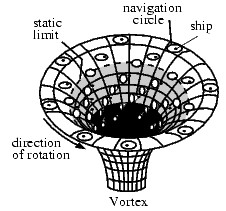
\includegraphics[width = 0.35\textwidth]{vortex}\\
\label{fig:vortex}
Искривление пространства-времени вблизи черной дыры.
\end{center}

На рисунке \ref{fig:vortex} показан так называемый водоворот черной дыры. Можно заметить глубокое сходство черной дыры и известного эффекта вихря - например, гигантского водоворота, порожденного морскими течениями. Объект, находящийся вблизи черной дыры, имеет 3 различных варианта продолжения движения в зависимости от расстояния до центра черной дыры. Белая зона на рисунке (\ref{fig:vortex}) показывает ту область пространства, в которой тело может двигаться произвольно относительно черной дыры: удаляться от черной дыры, двигаться в различных направлениях относительно вращения черной дыры (сонаправленно или противонаправлено).

Серая зона показывает ту область, где на направление движения тела имеются ограничения: В этой области тело не может двигаться против вращения черной дыры, но все еще может удалиться от нее, двигаясь по раскручивающейся спирали. Граница между Белой и Серой зоной получила название \textit{предел статичности.}

Черная зона показывает ту область, попав в которую тело уже никогда не сможет покинуть черную дыру. Граница между черной и серой зоной называется \textit{горизонт событий.}

Для черных дыр введено понятие массы-энергии:

\begin{equation}
M^{2} = \frac{J^{2}}{4M_{ir}^{2}} + \left(\frac{Q^{2}}{4M_{ir}} + M_{ir}\right)^{2},
\label{eq:mass-energy_equation}
\end{equation}

где $M_{ir} \equiv \frac{1}{2}\sqrt{\left(M + \sqrt{M^{2} - Q^{2} - a^{2}}\right)^{2} + a^{2}}$

В формуле (\ref{eq:mass-energy_equation}) первый член соответствует вращательной энергии, второй — кулоновской, а третий описывает так называемую неприводимую энергию черной дыры. 

Отдельно стоит отметить вклад кулоновской энергии. Для всех астрономических черных дыр можно пренебречь данной компонентой энергии, так как гравитационное притяжение намного слабее электромагнитного отталкивания заряженных частиц, то черная дыра, которая приобрела заряд Q, практически мгновенно его потеряет. 

Заметим, что площадь горизонта событий $A$ и неприводимая масса черной дыры связаны соотношением:

\begin{equation}
M_{ir} = \sqrt{\frac{A}{16\pi}}
\label{eq:mass_square_equation}
\end{equation}

Данной соотношение будет полезно при рассмотрении влияния вращательного движения черной дыры на ее энтропию.

Энтропия черной дыры определяется как:

\begin{equation}
S = \frac{k_{b}}{\hbar}\frac{A}{4}
\label{eq:entropy_equation}
\end{equation}


используя выражения (\ref{eq:entropy_equation}), (\ref{eq:mass_square_equation}) и (\ref{eq:mass-energy_equation}) получаем итоговую зависимость:

\begin{equation}
S\left(J\right) = \frac{2k_{b}\pi}{\hbar}\sqrt{2M\left(M + \sqrt{M^{2} - \left(\frac{J}{M}\right)^{2}}\right)}
\end{equation}

\section*{4.3}

\begin{center}
	\LARGE{\textbf{Лагранжиан стандартной модели.}}\\
\end{center}

\begin{equation*}
L = -\frac{1}{4} F_{\mu \nu} F^{\mu \nu} + i \overline{\psi} \cancel D \psi + h.c. + \psi_{i} y_{ij} \psi_{j} \phi + h.c. + |D_{\mu} \phi |^2 - V(\phi )
\end{equation*}

\section*{4.4}

\begin{center}
	\LARGE{\textbf{Чем отличается темная материя от темной энергии?}}\\
\end{center}

Тёмная материя — гипотетическая форма материи, не участвующая в электромагнитном взаимодействии и поэтому недоступная прямому наблюдению. Составляет порядка четверти массы-энергии Вселенной и проявляется только в гравитационном взаимодействии. Понятие тёмной материи введено для теоретического объяснения проблемы скрытой массы в эффектах аномально высокой скорости вращения внешних областей галактик и гравитационного линзирования (в них задействовано вещество, масса которого намного превышает массу обычной видимой материи); среди прочих предложенных оно наиболее удовлетворительно.\\

Тёмная энергия — гипотетический вид энергии, введённый в математическую модель Вселенной ради объяснения наблюдаемого её расширения с ускорением.
Существует три варианта объяснения сущности тёмной энергии:
\begin{enumerate}
	\item тёмная энергия есть космологическая константа — неизменная энергетическая плотность, равномерно заполняющая пространство Вселенной (другими словами, постулируется ненулевая энергия и давление вакуума).
	\item тёмная энергия есть некая квинтэссенция — динамическое поле, энергетическая плотность которого может меняться в пространстве и времени.
	\item тёмная энергия есть модифицированная гравитация на расстояниях порядка размера видимой части Вселенной.
\end{enumerate}


\section*{4.5}

\begin{center}
	\LARGE{\textbf{Как ведет себя линейная комбинация $\overrightarrow{M} \times \overrightarrow{v}$ и $\overrightarrow{\nabla}V(r)$?}}\\
\end{center}

Найдём значение производной линейной комбинации $$[\textbf{vM}] + \alpha \textbf{r}f(r),$$ где $\alpha \textbf{r}f(r) = grad (V(\textbf r))$ в центральном поле. Имеем:
$$[\mathbf{\dot{v}M}] + {\alpha \textbf{v}}f(r) + \frac {\alpha \textbf{r} (\textbf{vr})}{r}\frac {df(r)}{dr}.$$
Заметим, что при движении в полях $ U = \frac{\alpha}{r}$ (ньютоновские поля тяготения и кулоновские электростатические поля) с любым знаком $\alpha$  имеется интеграл движения, специфический именно для этого поля. 
Действительно, при $f(r) \sim \frac {1}{r}$  полная производная линейной комбинации по времени равна
$$[\mathbf{\dot{v}M}] + \frac {\alpha \textbf{v}}{r} - \frac {\alpha \textbf{r} (\textbf{vr})}{r^3},$$
или, подставив $\textbf{M} = m[\textbf{rv}]:$
$$m\mathbf{r(v\dot{v})} - m\mathbf{v(r\dot{v})} + \frac {\alpha \textbf{v}}{r} - \frac {\alpha \textbf{r} (\textbf{vr})}{r^3};$$
положив здесь согласно уравнениям движения $ m\mathbf{\dot{v}} = \frac {\alpha \textbf{r}}{r^3}$, мы найдём, что выражение (1) обращается в нуль.
Сохраняющийся вектор $$[\textbf{vM}] + \frac {\alpha \textbf{r}}{r}$$ направлен вдоль большой оси от фокуса к перигелию, а по величине равен $\alpha e$, где $e$ - эксцентриситет орбиты. Данная величина носит название "вектор Лапласа - Рунге - Ленца".

\section*{4.6}

\begin{center}
	\LARGE{\textbf{Решается ли уравнение $\left( x^{5}-a^{2}\right) ^{3}=b$ в радикалах и чему равна его группа Галуа?}}\\
\end{center}

\subsection*{Разрешимость}
Уравнение $\left( x^{5}-a^{2}\right) ^{3}=b$ разрешимо в радикалах. В качестве доказательства предоставим его решение:
\\$\left( x^{5}-a^{2}\right) ^{3}=b$
\\$x^{5}-a^{2}=\sqrt [3] {b}e^{\frac {2\pi in}{3}},n\in \left\{ 0,1,2\right\} $
\\$x^{5}=a^{2}+\sqrt [3] {b}e^{\frac {2\pi in}{3}},n\in \left\{ 0,1,2\right\} $
\\$x=\sqrt {a^{2}+\sqrt [3] {b}e^{\frac {2\pi in}{3}}}e^{\frac {2\pi im}{5}},n\in \left\{ 0,1,2\right\} ,m\in \left\{ 0,1,2,3,4\right\} $
\\Таким образом, найдены ровно 15 корней многочлена, который имеет степень, равную 15, то есть все корни выражены через радикалы.

\subsection*{Группа Галуа}
Как известно, уравнение разрешимо тогда и только тогда, когда его группа Галуа разрешима. Покажем это. Расширением Гаула будет являться $\mathbb {L/R}$, где $\mathbb{L} = \mathbb{K}(a ^{2}+\sqrt [3] {b}\left( 1-i\sqrt {3}\right), \: a ^{2}+\sqrt [3] {b}\left( 1+i\sqrt {3}\right)) $, а $\mathbb{K} = \mathbb{R}(i)$.
\\Поле $\mathbb{L}$ разрешимо, поскольку $\mathbb{L} \supseteq \mathbb{K} \supseteq \mathbb{R}$. Фактически, $\mathbb{L/K}$ и $\mathbb{K/Q}$ являются расширениями Галуа. Интересующая нас группа Гаула это $G(\mathbb{L/Q}) = S_4$. Известно также, что $S_n$ при $n < 5$ разрешима, таким образом уравнение действительно разрешимо в радикалах.

\section*{4.7}

\begin{center}
	\LARGE{\textbf{Конформационная структура белка - разные уровни и их роль.}}\\
\end{center}

Последовательность аминокислотных остатков в полипептидной цепи называется первичной структурой белка.
Цепочка из аминокислот не будет находиться в растворе в полностью вытянутой форме, обычно она складывается в более сложные структуры. Кислород группы C=O может образовывать водородную связь с водородом группы N-H, расположенной в другой аминокислоте. За счёт таких водородных связей формируется вторичная структура белка.\\
Укладка белков обычно не ограничивается вторичной структурой. Между аминокислотными остатками возникают различные слабые связи. Например, между -СОО$^-$-группами кислых аминокислот и NH3$^+$-группами лизина может возникнуть электростатическое притяжение. Между атомами кислорода или азота одних гидрофильных аминокислот и атомами водорода других могут образоваться водородные связи. Гидрофобные аминокислотные остатки "стремятся" укрыться от водного окружения внутри белковой молекулы. Некоторую роль играют также ван-дер-ваальсовы взаимодействия (они обеспечивают слабое притяжение любых атомов с электронными оболочками). Имеются и ковалентные связи, стабилизирующие третичную структуру белка, - это т. н. дисульфидные мостики -S-S-, образующиеся между двумя остатки аминокислоты цистеина: R-SH + R-SH - 2H = R-S-S-R. Благодаря всем этим взаимодействиям - гидрофобным, ионным, водородным, ван-дер-ваальсововым и дисульфидным - белковая цепочка образует сложную пространственную конфигурацию, называемую третичной структурой.\\
Многие белки (их называют олигомерными) состоят не из одной, а из нескольких полипептидных цепочек – так, белок крови гемоглобин состоит из четырех цепей. Совокупность их образует четвертичную структуру белка, при этом отдельные цепочки называются субъединицами. Четвертичная структура удерживается теми же связями, что и третичная. Пространственная конфигурация белка (т. е. его третичная и четвертичная структура) называется конформацией. Все более высокие уровни организации белковой молекулы определяются первичной структурой данного белка (постулат Полинга-Афинсена).

\section*{4.8}

\begin{center}
	\LARGE{\textbf{В чём состоит (утверждает) теория Калуцы-Клейна?}}\\
\end{center}

\subsection*{ Введение }

	К 1916 году Альберт Эйнштейн заканчивает создание Общей теории относительности, получившей впоследствии небывалый успех. Теория смогла предсказать множество не имеющих до этого момента обьяснения явлений, таких как "прецессия перигелия орбиты Меркурия" и "космологическое красное смещение". Элегантно обьединяя в себе уравнения гравитационного поля и уравнения движения, теория, тем не менее, никак не обьясняла наличие других фундаментальных взаимодействий. \\
	В апреле 1919 года А. Эйнштейн получает письмо малоизвестного математика Теодора Калуцы, в котором тот предлагает модель, претендующую на объединение ОТО и классической теории Максвелла. Последующая разработка этой теории множеством знаменитых учёных XX века привела к созданию первой внутренне непротиворечивой теории объединения, однако, не имевшевшей экспериментального подтверждения. Тем не менее, в дальнейшем идеи Калуцы нашли продолжение в дальнейшем.

\subsection*{ Основные идеи }

	 Основной идеей является предложение дополнить криволинейное пространство Эйнштейна компактным пятым измерением:

	\begin{align*}
	 	\tilde g_{ab} =
		\left( \begin{array}{cc}
			g_{ \mu \nu } + \phi^2 A_{\mu} A_{\nu} & \phi^2 A_{\mu}    \\
			\phi^2 A_{ \nu }                       & \phi^2            \\
		\end{array} \right)
	\end{align*}

	Где $ \tilde g_{ab} $ - пятимерный метрический тензор с латинскими индексами соответственно, $g_{ \mu \nu }$ - обычный четырёхмерный метрический тензор ОТО, индексируемый греческим алфавитом. Как мы увидим впоследствии, величины $A_{\mu}$ следует отождествлять с компонентами 4-потенциала электромагнитного поля.
	Тогда ковариантный метрический тензор

	\begin{align*}
	 	\tilde g^{ab} =
		\left( \begin{array}{cc}
			g^{ \mu \nu } & - A^{\mu}                                                  \\
			- A^{ \nu }   &  g_{\alpha \beta} A^{\alpha} A^{\beta} + \frac{1}{\phi^2}  \\
		\end{array} \right)
	\end{align*}

	Таким образом, метрика будет иметь вид:

	\begin{align*}
	 	ds^2 = \tilde g_{ab} dx^a dx^b = g_{\mu \nu} dx^{\mu} dx^{\nu} + \phi^2 (A_{\nu} dx^{\nu} + dx^5)^2
	\end{align*}

\subsection*{Уравнения поля в вакууме}

	Для упрощения уравнений обычно принимается условие цилиндра:

	\begin{align*}
	 	\frac{ \partial \tilde g_{ab} }{\partial x^5} = 0
	\end{align*}

	По аналогии с ОТО вводим символы Кристоффеля, тензор Риччи и действие для поля:

	\begin{align*}
	 	\tilde{\Gamma}_{bc}^a= \frac{1}{2} \tilde g^{ad} ( \partial_b \tilde g_{dc}& + \partial_c \tilde g_{db} - \partial_d \tilde g_{bc}) \\
	 	\tilde{R}_{ab} = \partial_c \tilde{\Gamma}_{ab}^c - \partial_b \tilde{\Gamma}_{ca}^c & + \tilde{\Gamma}_{cd}^c \tilde{\Gamma}_{ab}^d - \tilde{\Gamma}_{bd}^c \tilde{\Gamma}_{ac}^d \\
	 	S_g = \int \tilde{R}_{ab} & \tilde{g}^{ab} \sqrt{ |\tilde{g}| } d^5 x
	\end{align*}

	Варьрование этой части действия даёт

	\begin{align*}
	 	\tilde{R}_{ab} - \frac{1}{2} \tilde g_{ab} \tilde R = 0
	\end{align*}

	Или в четырёхмерной форме:

	\begin{align*}
	 	{R}_{\mu \nu} - \frac{1}{2} g_{\mu \nu} R = \frac{1}{2} \phi^2 ( g^{\alpha \beta } F_{\mu \alpha} F_{\nu \beta} - \frac{1}{4} g_{\mu \nu} F_{\alpha \beta} F^{\alpha \beta} ) + \frac{1}{\phi}(\nabla_{\mu} \nabla_{\nu} \phi - g_{\mu \nu} \Box \phi)
	\end{align*}

	Где $ F_{\mu \nu} = \partial_{\mu} A_{\nu} - \partial_{\nu} A_{\mu} $

	Заметим, что при выборе $\phi$ в качестве постоянной левая часть уравнения переходит в тензор энергии - импульса электромагнитного поля, т. е. уравнение находится в полном соответствии с уравнениями Эйнштейна в вакууме.

\subsection*{Уравнения движения}

	Определим 5-скорость:

	\begin{align*}
	 	\tilde{U}^a = \frac{dx^a}{ds}
	\end{align*}

	Уравнения движения примут вид:

	\begin{align*}
	 \tilde{U}^b \nabla_b \tilde{U}^a = \frac{d \tilde{U}^a}{ds} + \tilde{\Gamma}_{bc}^a \tilde{U}^b \tilde{U}^c
	\end{align*}

	Можно показать, что данные уравнения содержат в себе как и движение в электромагнитном поле в общей теории относительности, так и силу Лоренца. Не менее интересен ещё один результат, непосредственно вытекающий из данной системы. Выполнение уравнений движения требует того, чтобы удельный заряд частиц $ \frac{q}{m} $ был пропорционален $ \frac{dx^5}{ds_4} $, где в данном случае под $ ds_4 $ подразумевается $ ds_4 = g_{\mu \nu} dx^{\mu} dx^{\nu} $ четырёхмерный интервал. Таким образом, мы получаем, что заряд частицы определяется "скоростью" её движения в пятом измерении.


\subsection*{Тензор энергии-импульса}

	В заключение, нужно определить тензор энергии-импульса материи. По аналогии с СТО и ОТО 

	\begin{align*}
	 	\tilde{T}^{ab} = \rho \frac{dx^a}{ds} \frac{dx^b}{ds}
	\end{align*}

	Сравнивая результат такого определения с ОТО, мы понимаем, что пространственные компоненты дают обычным тензор энергии частиц, а компоненты вида $ T^{5 \mu} $ следуют отождествить с энергией электромагнитного поля этих частиц.

\subsection*{Cкалярное поле}

	В течение всего обзора мы никак не акцентировали внимание на роли, которую играет в этой теории велицина $ \phi $ составляющая некоторое скалярное поле. Выбирая её константой, мы ограничиваем "электромагнитное поле", так как на связь $ \phi $ и $ F_{\mu \nu} $ существуют дополнительные уравнения. Данный факт не был учтён в ранних работах Калуцы-Клейна, что представляло собой некоторое заблуждение. 

	До сих пор нужное скалярное поле не было обнаружено экспериментально, из-за чего теорию нельзя считать подтверждённой.

\subsection*{Развитие}

	На данный момент гипотеза Калуцы-Клейна не считается перспективной, однако, в своё время она послужила началом постороения многомерных теорий объединения и теорий супергравитаций, таких как теория струн или М - теория.


\section*{4.9}

\begin{center}
	\LARGE{\textbf{Что такое джозефсоновский контакт?}}\\
\end{center}

\begin{center}
	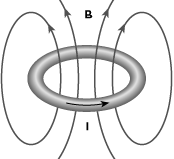
\includegraphics[width=0.3\textwidth]{4_9_0}\\
	Рис. 1.\\
	Незатухающий ток и создаваемое им магнитное поле не могут иметь произвольную величину, они квантуются так, что магнитный поток, пронизывающий кольцо, принимает значения, кратные элементарному кванту потока
\end{center}

Туннельный эффект - это типичная задача квантовой механики. Частица (например, электрон в металле) подлетает к барьеру (например, к слою диэлектрика), преодолеть который она по классическим представлениям никак не может, так как ее кинетическая энергия недостаточна, хотя в области за барьером она со своей кинетической энергией вполне могла бы существовать. Напротив, согласно квантовой механике, прохождение барьера возможно. Частица с некоторой вероятностью может как бы пройти по туннелю через классически запрещенную область, где ее потенциальная энергия как бы больше полной, то есть классическая кинетическая энергия как бы отрицательна. На самом деле с точки зрения квантовой механики для микрочастицы (электрона) справедливо соотношение неопределенностей $\Delta x \Delta p > h$ (x - координата частицы, p - ее импульс). Когда малая неопределенность ее координаты в диэлектрике $\Delta x = d$ (d-толщина слоя диэлектрика) приводит к большой неопределенности ее импульса $\Delta p \ge h / \Delta x$, а следовательно, и кинетической энергии $p^2/(2m)$ (m - масса частицы), то закон сохранения энергии не нарушается. Опыт показывает, что действительно между двумя металлическими обкладками, разделенными тонким слоем диэлектрика (туннельный переход), может протекать электрический ток тем больший, чем тоньше диэлектрический слой.\\
Джозефсон рассматривал частный случай туннельного эффекта - туннелирование куперовских пар - и предсказал существование двух эффектов. Первый из них состоит в том, что через туннельный переход с тонким слоем диэлектрика, когда его толщина меньше или порядка длины когерентности,  возможно протекание сверхпроводящего тока, то есть тока без сопротивления. Это стационарный эффект Джозефсона. Предсказывалось, что критическое значение этого тока будет своеобразно зависеть от внешнего магнитного поля. Если ток через такой переход станет больше критического, то переход будет источником высокочастотного электромагнитного излучения. Это нестационарный эффект Джозефсона.\\
Понадобилось немного времени, чтобы обнаружить эти эффекты экспериментально. Более того, вскоре стало ясно, что эффекты Джозефсона присущи не только туннельным переходам, но и более широкому классу объектов - сверхпроводящим слабым связям, то есть участкам сверхпроводящей цепи, в которых критический ток существенно подавлен, а размер участка порядка длины когерентности.\\
В основе эффектов Джозефсона лежат квантовые свойства сверхпроводящего состояния. Действительно, сверхпроводящее состояние характеризуется когерентностью куперовских пар: эти пары электронов находятся на одном квантовом уровне и описываются общей для всех пар волновой функцией, ее амплитудой и фазой. Они когерентны как частицы света - фотоны в излучении лазера, которое также характеризуется амплитудой и фазой электромагнитной волны.\\
Представим теперь себе два массивных куска одного и того же сверхпроводника, полностью изолированных друг от друга. Так как оба они находятся в сверхпроводящем состоянии, каждый из них будет характеризоваться своей волновой функцией. Поскольку материалы и температуры одинаковы, модули обеих волновых функций должны совпадать, а фазы произвольны. Однако, если установить между ними хотя бы слабый контакт, например туннельный, куперовские пары будут проникать из одного куска в другой и установится фазовая когерентность. Возникнет единая волновая функция всего сверхпроводника, которую можно рассматривать как результат интерференции волновых функций двух половинок.
Представим теперь себе два массивных куска одного и того же сверхпроводника, полностью изолированных друг от друга. Так как оба они находятся в сверхпроводящем состоянии, каждый из них будет характеризоваться своей волновой функцией. Поскольку материалы и температуры одинаковы, модули обеих волновых функций должны совпадать, а фазы произвольны. Однако, если установить между ними хотя бы слабый контакт, например туннельный, куперовские пары будут проникать из одного куска в другой и установится фазовая когерентность. Возникнет единая волновая функция всего сверхпроводника, которую можно рассматривать как результат интерференции волновых функций двух половинок.
\subsection*{Квантовая интерференция}

Уже в первом эксперименте было обнаружено, что максимальный сверхпроводящий ток $I_c$ в магнитном поле, параллельном плоскости контакта, немонотонно зависит (с периодом, равным кванту потока $\Phi_0$) от величины магнитного потока $\Phi$, проникающего в контакт. Эта зависимость показана тут:

\begin{center}
	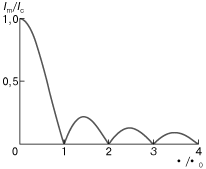
\includegraphics[width=0.3\textwidth]{4_9_1}\\
	Рис. 2.\\
	Зависимость критического тока $I_m$ (нормированного на критический ток при отсутствии поля $I_c$) джозефсоновского контакта от величины потока внешнего магнитного поля.
\end{center}

Как видно из рисунка, в случае, когда поток равен целому числу квантов $\Phi_0$, происходит компенсация токов, текущих в противоположные стороны в разных точках контакта, и результирующий критический ток оказывается равным нулю. Этот график аналогичен зависимости интенсивности света на экране при дифракции на одиночной щели от расстояния до центральной точки и наглядно демонстрирует волновые свойства сверхпроводящих токов.

Чтобы рассмотрение этого явления стало более простым, включим туннельный контакт в сверхпроводящий контур (кольцо). Магнитный поток через площадь сверхпроводящего кольца (не содержащего контакта) строго постоянен. Его значение, как уже говорилось, квантуется. Оно равно целому числу квантов $\Phi_0$, и изменить его, не переводя кольцо в нормальное состояние, невозможно. Но если кольцо содержит слабую связь, то магнитный поток может меняться - кванты потока проникают в контур через это слабое место. 
Посмотрим, как при изменении внешнего магнитного поля меняется величина потока $\Phi$ и тока $I$ в кольце со слабой связью. Пусть сначала внешнее поле и ток в контуре равны нулю (рис. 3, а). Поток $\Phi$ при этом тоже равен нулю. Увеличим внешнее поле - по закону индукции Фарадея в контуре появится сверхпроводящий ток, своим магнитным полем по закону Ленца компенсирующий внешний поток. Так будет происходить, пока ток в контуре не станет равным критическому току контакта $I_c$ (рис. 3, б ). Для простоты рассмотрения выберем площадь кольца такой, чтобы при $I = I_c$ внешнее поле создавало поток $\Phi$, равный половине кванта потока: $\Phi = \Phi_0 / 2$.
\begin{center}
	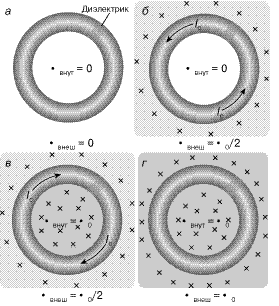
\includegraphics[width=0.3\textwidth]{4_9_2}\\
	Рис. 3.\\
	Сверхпроводящий контур с джозефсоновским элементом во внешнем магнитном поле.
\end{center}
\begin{center}
	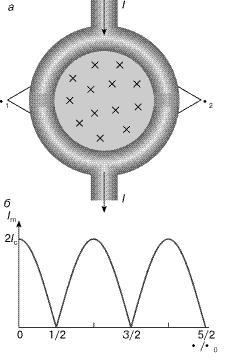
\includegraphics[width=0.3\textwidth]{4_9_3}\\
	Рис. 3.\\
	Сверхпроводящий контур с джозефсоновским элементом во внешнем магнитном поле.
\end{center}
Как только ток станет больше $I_c$ , сверхпроводимость в контакте нарушится и в контур войдет квант потока $\Phi_0$ (рис. 3, в). При этом отношение $\Phi / \Phi_0$ скачком увеличится на единицу, а направление тока изменится на противоположное, хотя его величина останется прежней $I_c$ . Действительно, если до вхождения кванта потока $\Phi_0$ ток $I_c$ полностью экранировал внешний поток $\Phi = \Phi_0 / 2$, то после вхождения он должен усиливать внешний поток $\Phi_0 / 2$ до значения $\Phi_0$. Таким образом, контур перешел в новое квантовое состояние.
При дальнейшем увеличении внешнего поля ток в кольце будет уменьшаться, а поток будет оставаться равным $\Phi_0$. Ток обратится в нуль, когда внешний поток станет равным $\Phi_0$(рис. 3, г), а затем ток потечет в обратном направлении, частично экранируя внешний поток. При внешнем потоке $3 \Phi_0 / 2$ ток опять станет равным $I_c$ , сверхпроводимость нарушится, войдет следующий квант потока и т.д. Ступенчатый характер рассмотренных зависимостей позволяет почувствовать отдельные кванты потока, а ведь эта величина очень мала, всего лишь порядка $2 \cdot 10^{-15}$Вб. 
Особенно ярко когерентные свойства сверхпроводящего состояния проявляются при включении в контур двух джозефсоновских контактов (рис. 4, а). Полный ток I при этом определяется интерференцией токов, протекающих через контакты: 
\begin{equation*}
	I_m = I_c sin \varphi_1 + I_c sin \varphi_2,
\end{equation*}

где $\varphi_1$ и $\varphi_2$ - скачки фаз волновых функций на переходах, а критические токи обоих контактов для простоты взяты одинаковыми и равными $I_c$. 

В результате критический ток $I_m$ периодически зависит от внешнего магнитного поля и обращается в нуль, когда поток равен полуцелому числу квантов (рис. 4, б ). Эта зависимость в точности соответствует оптическому аналогу - зависимости интенсивности света на экране от расстояния при дифракции на двух щелях. 
    
Применение 
Экспериментальные образцы приборов с контактом Джозефсона могут обнаруживать напряжения порядка $10^{–15}$В.  Магнитометры, способные обнаруживать магнитные поля порядка $10^{–13}$Тл, используются при изучении магнитных материалов, а также в медицинских магнитокардиографах. Чрезвычайно чувствительные детекторы вариаций силы тяжести могут применяться в различных областях геофизики. 
Техника сверхпроводимости и особенно контакты Джозефсона оказывают все большее влияние на метрологию. С помощью джозефсоновских контактов создан стандарт $1$ В (об этом ниже). Был разработан также первичный термометр для криогенной области, в которой резкие переходы в некоторых веществах используются для получения реперных (постоянных) точек температуры. Новая техника используется в компараторах тока, для измерений радиочастотной мощности и коэффициента поглощения, а также для измерений частоты. Она применяется также в фундаментальных исследованиях, таких, как измерение дробных зарядов атомных частиц и проверка теории относительности.

Сверхпроводниковый суперкомпьютер
Идея использования джозефсоновских переходов в качестве элементной базы компьютеров появилась уже довольно давно. И если задача получения малых размеров переходов (плотность упаковки) и малого тепловыделения (в сверхпроводящем состоянии тепло вообще не рассеивается) довольно легко решается, то сверхвысокого быстродействия достичь долго не удавалось. 
Принципиально новое решение этой проблемы было впервые предложено в группе профессора К.К. Лихарева в МГУ. Для обработки и запоминания информации здесь используется квант магнитного потока, то есть нуль и единица - отсутствие или наличие в джозефсоновской ячейке одного кванта потока. Логические элементы с джозефсоновскими переходами, в которых проводится квантование магнитного потока, называются квантронами. Расчеты и эксперименты показывают, что квантроны обладают очень высоким быстродействием, достигающим значений $10^{12}$ операций в секунду. Однако они не подчиняются традиционным правилам схемотехники и их следует применять в схемах нового типа. Здесь информация передается от одного элемента к другому с помощью кванта магнитного потока, поэтому обязательным условием является близкое расположение элементов. Характерные расстояния, разделяющие при этом элементы, достигают величин порядка десятых долей микрона. Такие схемы выгодно применять, например, при создании регистров сдвига - устройств с передачей информации вдоль периодической структуры элементов логики, причем информация смещается на единичный период при введении или изъятии единичного кванта потока.
Установка на основе эффекта Джозефсона для воспроизведения единицы напряжения постоянного тока

Во ВНИИФТРИ создана установка на основе матрицы джозефсоновских переходов для воспроизведения единицы напряжения постоянного тока. 
Установка предназначена для калибровки и поверки многоразрядных аналого-цифровых преобразователей (АЦП) в интегральном исполнении, может также использоваться для калибровки и поверки высокоточных мер напряжения и цифровых вольтметров. 
Основным элементом установки является матрица джозефсоновских переходов, изготовленная в РТВ (Германия). Использование эффекта Джозефсона обеспечивает высокую точность воспроизведения напряжения. 
Установка состоит из криозонда с джозефсоновской матрицей, СВЧ генератора (длина волны ~ $4$ мм) с системой фазовой автоподстройки частоты, рубидиевого стандарта частоты, характериографа, транспортируемого гелиевого дюара. 

\section*{4.10}

\begin{center}
	\LARGE{\textbf{Сколько энтропии может вместить данный объем?}}\\
\end{center}

Для ответа на этот вопрос используем вероятностное определение энтропии. Энтропией системы называется сумма произведений вероятностей различных состояний системы на логарифмы этих вероятностей, взятая с обратным знаком: 
$$ H(X) = -\sum_{i=1}^n p_i\log p_{i}$$где X - некоторая случайная величина.

В таком случае, энтропия системы будет максимальна, когда все возможные состояния системы равновероятны. В таком случае $\forall i \quad p_{i} = \frac{1}{n},\qquad H = \log n$

В данной формуле логарифм может быть взят по любому основанию, выбор основания влияет непосредственно на системы единиц, в которых будут выражены Физические величины. 

Связь данной формулы с объемом заключается в том, что если заранее ограничить некоторый объем пространства, которое занимает физическая система, то можно описать все состояния, в которых система может находиться внутри данного объема, так как количество таких состояний конечно. Если бы количество состояний, в которых может находиться система было бесконечно, то принципиально нельзя было бы описывать поведение физических систем, по причине того, что на любое внешнее воздействие система могла бы реагировать каждый раз по новому. Таким образом, даже при отсутствии внешнего воздействия нельзя бы было описать систему, ведь в таком случае вероятность каждого события стремится к нулю, чего не может быть на самом деле.

В итоге: ограниченный объем влияет на количество всевозможных состояний, в которых может находиться система, а зная количество таких состояний и вероятность нахождения в системы в каждом из них можно определить энтропию системы.

\section*{5.3}

\begin{center}
	\LARGE{\textbf{Почему уравнения движения для фермионов первого порядка?}}\\
\end{center}

Движение фермионов описывается уравнениями Дирака, которые являются релятивистским обобщением \textbf{уравнения Шредингера}:
\begin{equation}
	i \hbar \frac{\partial}{\partial t} \Psi=\hat{H}(p, q) \Psi
\end{equation}
В уравнении Шредингера стоит первая производная по времени, потому что по теореме Нетер гамиальтониан-величина, сохраняющаяся при инвариантости системы относительно трансляций по времени (а генератором трансляций по времени выступает оператор производной по времени).\\
Однако уравнение Шредингера не удовлетворяет принципам СТО так как оно не инвариантно относительно преобразований Лоренца (тк вторые производные по координатам и первая по времени). Поэтому его релятивистское обобщение имеет вид:
\begin{equation}
	i \hbar \frac{\partial \psi}{\partial t}=\left[c\left(\alpha_{x} \frac{\partial}{\partial x}+\alpha_{y} \frac{\partial}{\partial y}+\alpha_{z} \frac{\partial}{\partial z}\right)+\beta m c^{2}\right] \psi.
\end{equation}


\section*{5.4}

\begin{center}
	\LARGE{\textbf{Как находят экзопланеты?}}\\
\end{center}

Один из способов -- метод транзитов. Проводятся наблюдение за яркостью звёзд, чтобы среди тех, которые изменяют её периодично, выявить звёзды с экзопланетами (если лоскость орбиты \textit{почти} содержит луч зрения, то планета будет периодически проходить по диску звезды). С помощью этого метода обнаружено подавляющее большинство известных на сегодня экзопланет, в частности, именно этим методом в основном искал планеты телескоп Кеплер. Второй способ, с отрывом являвшийся наиболее используемым до появления т. Кеплер -- наблюдение за лучевой скоростью звезды (из-за движения звезды вокруг центра масс системы лучевая скорость меняется со временем, из-за чего линии в её спектре движутся). Точность лучших современных спектрометров в некоторых случаях позволяет обнаружить флуктуации лучевой скорости даже меньшие, чем 3$\frac{m}{s}$. Поиск планет при микролинзировании -- ещё один способ, появившийся относительно недавно. Если одна звезда выступает как грав. линза для света другой далёкой звезды, то возможная планета у линзирующей звезды изменит изображение. Наконец, существует метод прямого наблюдения -- когда планету удаётся обнаружить на снимке (звезда при этом закрывается коронографом). Существуют и другие методы, которые, однако, практически не используются. Методы, естественно, комбинируются: не редко земным спектрометром измеряют лучевую скорость у звезды, попавшей в список кандидатов на наличие планеты благодаря транзитным наблюдениям на космическом телескопе.

\section*{5.5}

\begin{center}
	\LARGE{\textbf{Когда и почему постоянна скорость прецессии?}}\\
\end{center}

Вынужденная прецессия гироскопа вызывается моментом внешних сил, поворачивающих момент импульса гироскопа, согласно уравнению
\begin{equation}
    \dot{\vec{L}} = \vec{M}.
    \label{equation}
\end{equation}
Момент импульса гироскопа, равный $\vec{L} = \hat{I} \vec{\omega}$, можно разложить по друм осям:
$$
\vec{L} = I_{||} \vec{\omega}_{||} + I_{\perp} \vec{\omega}_{\perp},
$$
где $I_{||} \vec{\omega}_{||}$ -- компонента вектора импульса, направленная вдоль оси фигуры гироскопа, а $I_{\perp} \vec{\omega}_{\perp}$ -- вдоль оси, перпендикулярной к оси фигуры.

В приближённой теории гироскопа мы считаем, что $I_{||} \omega_{||} \gg I_{\perp} \omega_{\perp}$ (гироскоп быстро вращается вокруг оси фигуры), и, как следствие, $\vec{L} \approx I_{||} \vec{\omega}_{||} \approx I_{||} \vec{\omega}$, т.е. $\vec{L}$ и $\vec{\omega}$ сонаправлены.
\\
Пусть внешняя сила $\vec{F}$ приложена к точке, лежащей на оси фигуры гироскопа; $\vec{r}$ -- радиус-вектор, проведённый от точки опоры гироскопа к точке приложения силы $\vec{F}$. Момент этой силы будет равен $\vec{M} = [\vec{r},\vec{F}]$. Тогда, в силу уравнения (\ref{equation}), $\dot{\vec{L}}$ будет перпендикулярен к оси фигуры, т.е. под влиянием момента внешней силы будет изменяться направление $\vec{L}$, а не его модуль -- это и есть явление прецессии. Найдём угловую скорость $|\vec{\omega}_{пр}|$ этого вращения.
\\
Так как $\vec{L}$ изменяется не по модулю, а только по направлению, то можем представить, что $\vec{L}$ -- радиус-вектор некоторой точки. Тогда линейная скорость этой точки $\dot{\vec{L}}$ будет равна $[\vec{\omega}_{пр}, \vec{L}]$, отсюда получаем
$$
[\vec{\omega}_{пр}, \vec{L}] = \vec{M}.
$$
Пусть $\vec{\omega}_{пр}$ составляет угол $\alpha$ с $\vec{L}$. Тогда
$$
\omega_{пр} L sin \alpha = M = r F sin \alpha
$$
$$
\omega_{пр} = \frac{r F}{L} = \frac{r F}{I_{||} \omega}.
$$
Отсюда ясно, что $\omega_{пр} = const$, когда $\frac{r F}{I_{||} \omega} = const$.

Приведённое выше рассуждение справедливо для быстро вращающегося гироскопа, т.е. $\omega_{||} \gg \omega_{\perp}, \omega_{пр}$. При медленном вращении нутационные колебания (колебания оси около её среднего направления) могут быть довольно заметными и, слагаясь с прецессией, существенно изменить движение оси: конец оси будет описывать ясно видимую волнообразную или петлеобразную кривую, то отклоняясь от вертикали, то приближаясь к ней.

\section*{5.6}

\begin{center}
	\LARGE{\textbf{Когда у двух полиномов есть общий корень?}}\\
\end{center}

Когда определитель их матрицы Сильвестра равен 0.

\section*{5.7}

\begin{center}
	\LARGE{\textbf{Что считается причиной болезни Альцгеймера?}}\\
\end{center}

В настоящий момент не установлены причины болезни Альцгеймера, однако существуют несколько основных конкурирующих гипотез:

1. Амилоидная гипотеза Согласно амилоидной гипотезе, причиной заболевания являются отложения бета-амилоида, вызывающие образование нейрофибриллярных клубков, гибель нейронов, и, как следствие – развитие деменции. Ген, кодирующий белок APP, из которого образуется бета-амилоид, расположен на 21 хромосоме. В поддержку данной гипотезы говорит тот факт, что у преобладающей части доживших до 40 лет больных Синдромом Дауна (дополнительная копия 21 хромосомы либо ее участка) обнаруживается сопутствующая Альцгеймеро-подобная патология.

2. Тау-гипотеза

Согласно тау-гипотезе, нарушения в работе головного мозга связаны с отклонениями в структуре тау-белка, вызывающими разрушение транспортной системы внутри нейрона, приводя к гибели клеток.

3.Холинергическая гипотеза

Первая из предложенных гипотез, согласно которой болезнь вызывается сниженным синтезом нейромедиатора ацетилхолина, однако сейчас считается маловероятной ввиду того, что медикаменты, способные скорректировать уровень ацетилхолина, имеют низкую эффективность.

4. Инфекционная гипотеза

Новейшая из основных гипотез, предполагающая связь болезни Альцгеймера с возбудителем периодонтита – болезни, связанной с воспалением соединительной ткани в щелевидном пространстве зуба. Возбудитель был обнаружен в мозге людей, погибших от болезни Альцгеймера; кроме того, в экспериментах на мышах эта инфекция приводила к колонизации мозга бактериями и увеличению вырабатывания бета-амилоида, ассоциируемого с болезнью Альцгеймера.

Таким образом, наиболее вероятными причинами болезни Альцгеймера можно считать отложения бета-амилоида и/или деятельности в мозге возбудителя периодонтита.

\section*{5.8}

\begin{center}
	\LARGE{\textbf{Что такое конфайнмент? (в т.ч. формулы для межкварковой силы и вильсоновского среднего)?}}\\
\end{center}

Конфайнмент – явление в физике элементарных частиц, состоящее в невозможности получения кварков в свободном состоянии – в эксперементах наблюдаются только частицы, состоящие из двух (мезоны), трех (барионы), четырех (тетракварки) и пяти (пентакварки) кварков. Кварки в пределах адрона не могут удалиться друг от друга на расстояние, заметно превышающее радиус конфайнмента (порядка 1фм).

Связь Вильсоновского среднего и Конфайнмента:
\begin{center}
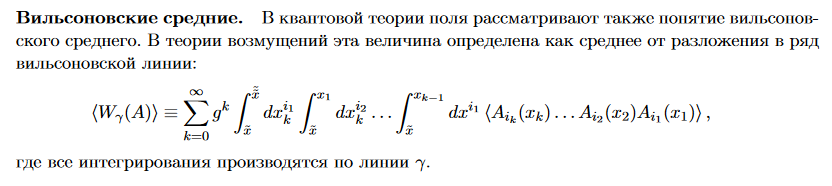
\includegraphics[width=1.00\textwidth]{5_8_0}
\end{center}

В "Элементарное введение в физику элементарных частиц, Окунь Л.Б., 1985." на тему межкварковой силы написано:
В гравитации и электродинамике мы привыкли к тому, что силы между частицами растут, когда частицы сближаются, и ослабевают, когда частицы расходятся (потенциалы типа $1/r$). В случае кварков ситуация другая. Имеется критический радиус $r_0~=10^{-13}$ см, при $r<<r_{0}$ потенциал похож на кулоновский или ньютоновский,но при $r>~r_0$ его поведение резко меняется – он начинает стремительно расти.

\section*{5.9}

\begin{center}
	\LARGE{\textbf{Что такое космическая цензура?}}\\
\end{center}

Принцип <<космической цензуры>> был сформулирован в 1970 году Роджером Пенроузом в следующей образной форме: <<Природа питает отвращение к голой сингулярности>>. Формулировка Пенроуза предполагает, что пространство-время в целом является глобально гиперболическим. Горизонт событий чёрной дыры является световой поверхностью, образующие которой при продолжении их в будущее никогда не пересекаются между собой. В таких областях становится неприменимым базовое приближение большинства физических теорий, в которых пространство-время рассматривается как гладкое многообразие без края. Часто в гравитационной сингулярности величины, описывающие гравитационное поле, становятся бесконечными или неопределёнными. К таким величинам относятся, например, скалярная кривизна или плотность энергии в сопутствующей системе отсчёта. В классической чёрной дыре в сингулярности сила гравитации настолько велика, что свет не может покинуть горизонт событий и, таким образом, объекты внутри горизонта событий, включая саму чёрную дыру, не могут наблюдаться непосредственно.
\\ До осени 2017 года были основания сомневаться в его абсолютной правильности (например, коллапс пылевого облака с большим угловым моментом приводит к <<голой сингулярности>>, но неизвестно, стабильно ли это решение уравнений Эйнштейна относительно малых возмущений начальных данных). В своей работе, опубликованной в октябре 2017 года, математики Михалис Дафермос и Джонатан Лак доказали, что сильная форма космической цензуры, относящаяся к странной структуре чёрных дыр, неверна.
\\ В 2019 году американский физик Уильям Ист численно смоделировал коллапс вытянутого эллипсоида, заполненного пылью, и показал, что гипотеза космической цензуры в этом случае не нарушается, как это предполагалось ранее. Оказалось, что вместо голых сингулярностей при коллапсе в материи формируются каустики, а все сингулярности в конце концов накрываются горизонтом событий.
\\ Несмотря на то, что Общая теория относительности (ОТО) описывает большинство наблюдаемых гравитационных явлений, она не является полной. Одна из самых больших проблем ОТО — существование гравитационных сингулярностей, в которых кривизна пространства-времени обращается в бесконечность. В частности, такие сингулярности возникают в центре черной дыры Шварцшильда. Очевидно, что для описания процессов в окрестности сингулярности нужно учитывать не только гравитационные, но и квантовые эффекты. Грубо говоря, чем ближе мы подходим к сингулярности, тем больше рождается виртуальных частиц, которые, в свою очередь, искривляют пространство-время и разрушают исходную геометрию. К сожалению, физики до сих пор так и не построили Теорию Всего, которая объединила бы ОТО и Квантовую теорию поля. Поэтому никто не знает, как выглядит сингулярность на самом деле.

\section*{5.10}

\begin{center}
	\LARGE{\textbf{Как (и почему так) меняется плотность атмосферы с высотой? (указать разные приближения)}}\\
\end{center}

\begin{enumerate}
    \item Изотермическая атмосфера.
    Принимая температуру и ускорение свободного падения постоянными, а атмосферу - находящейся в динамическом равновесии, получим:
    $$\rho (h) = \rho_0 \exp\left[-\frac{\mu g h}{RT}\right].$$
    Эта модель не учитывает изменения температуры атмосферы с высотой.
    
    \item Адиабатическая атмосфера.
    В модели адиабатической атмосферы в динамическом равновесии, плотность зависит от высоты так:
    $$\rho (h) = \rho_0 \left(1 - \frac{\gamma - 1}{\gamma} \frac{\mu g h}{R T_0}\right)^{1/(\gamma - 1)}.$$
    В этой модели температура линейно падает с высотой. В этой модели атмосфера должна закончиться на тридцати километрах над уровнем моря. Однако, на гораздо больших высотах наблюдаются метеоры и серебристые облака. Эта модель не учитывает отклонение зависимости температуры от высоты от прямой.
    
    \item Обе формулы выше плохо описывают плотность атмосферы на больших высотах. Температура атмосферы зависит от высоты нетривиальным образом. Для более хорошего описания атмосферы существуют более точные модели, например, International Standard Atmosphere или US Standard Atmosphere. Фактически, эти модели представляют собой кусочно заданные функции, учитывающие сложное поведение зависимости температуры от высоты.
    
    Источник: Wikipedia.
\end{enumerate}

\end{document}